\documentclass[
	fontsize=10pt,
	twoside=true,
	open=any,
	%chapterprefix=true,
	%chapterentrydots=true,
	numbers=noenddot,
	%draft=true,
	%overfullrule=true,
]{kaobook}

% Set the language
\usepackage[english]{babel} % Load characters and hyphenation
\usepackage[english=british]{csquotes} % English quotes
\usepackage[utf8]{inputenc}

% Load packages for testing
\usepackage{blindtext}
%\usepackage{showframe} % Uncomment to show boxes around the text area, margin, header and footer
%\usepackage{showlabels} % Uncomment to output the content of \label commands to the document where they are used

% Load the bibliography package
\usepackage{styles/kaobiblio}
%\addbibresource{main.bib} % Bibliography file

% Load mathematical packages for theorems and related environments. NOTE: choose only one between 'mdftheorems' and 'plaintheorems'.
\usepackage{styles/mdftheorems}
%\usepackage{styles/plaintheorems}

\usepackage{color}

\usepackage{listings}
\lstset{ % General setup for the package
    language=Perl,
    basicstyle=\small\sffamily,
    numbers=left,
    numberstyle=\tiny,
    frame=tb,
    tabsize=4,
    columns=fixed,
    showstringspaces=false,
    showtabs=false,
    keepspaces,
    commentstyle=\color{red},
    keywordstyle=\color{blue}
}
\lstdefinestyle{numbers}{numbers=left, stepnumber=1, numberstyle=\tiny, numbersep=10pt}
\lstdefinestyle{nonumbers}{numbers=none}
% https://tex.stackexchange.com/questions/261748/filename-in-line-0-of-a-lstlisting#262294

\graphicspath{{examples/documentation/images/}{images/}} % Paths in which to look for images

\makeindex[columns=3, title=Alphabetical Index, intoc] % Make LaTeX produce the files required to compile the index

\makeglossaries % Make LaTeX produce the files required to compile the glossary

\makenomenclature % Make LaTeX produce the files required to compile the nomenclature

% English adjutants
\renewcommand{\eg}{\emph{e.g.,}}

% keystrokes
\newcommand{\CtrlC}{\texttt{Ctrl}+\texttt{C}}
\newcommand{\CtrlD}{\texttt{Ctrl}+\texttt{D}}
\newcommand{\CtrlZ}{\texttt{Ctrl}+\texttt{Z}}

% vanes
\newcommand{\ames}{\texttt{\%ames}}
\newcommand{\behn}{\texttt{\%behn}}
\newcommand{\clay}{\texttt{\%clay}}
\newcommand{\dill}{\texttt{\%dill}}
\newcommand{\eyre}{\texttt{\%eyre}}
\newcommand{\ford}{\texttt{++ford}}
\newcommand{\gall}{\texttt{\%gall}}
\newcommand{\iris}{\texttt{\%iris}}
\newcommand{\jael}{\texttt{\%jael}}
\newcommand{\lull}{\texttt{\%lull}}
\newcommand{\zuse}{\texttt{\%zuse}}

% common referents
\newcommand{\ask}{\texttt{\%ask}}
\newcommand{\chome}{\texttt{\%home}}
\newcommand{\ckids}{\texttt{\%kids}}
\newcommand{\graphstore}{\texttt{\%graph-store}}
\newcommand{\mock}{\texttt{++mock}}
\newcommand{\say}{\texttt{\%say}}
\newcommand{\unix}{\texttt{\%unix}}
\newcommand{\zod}{\texttt{\textasciitilde zod}}

% Hoon auras
\newcommand{\nullchr}{\texttt{\textasciitilde}}
\newcommand{\patc}{\texttt{@c}}
\newcommand{\patp}{\texttt{@p}}
\newcommand{\patt}{\texttt{@t}}
\newcommand{\patta}{\texttt{@ta}}
\newcommand{\pattas}{\texttt{@tas}}
\newcommand{\patub}{\texttt{@ub}}
\newcommand{\patud}{\texttt{@ud}}
\newcommand{\patux}{\texttt{@ux}}

\newcommand{\ub}{${0b}$}
\newcommand{\uc}{${0c}$}
\newcommand{\ui}{${0i}$}
\newcommand{\ux}{${0x}$}

\newcommand{\yes}{\texttt{\%.y}}
\newcommand{\no}{\texttt{\%.n}}

\newcommand{\irrtis}{\texttt{=(a b)}}

% core types
\newcommand{\gold}{\texttt{\%gold}}
\newcommand{\iron}{\texttt{\%iron}}
\newcommand{\lead}{\texttt{\%lead}}
\newcommand{\zinc}{\texttt{\%zinc}}

% ++move
\newcommand{\pass}{\texttt{\%pass}}
\newcommand{\give}{\texttt{\%give}}
\newcommand{\slip}{\texttt{\%slip}}
\renewcommand{\unix}{\texttt{\%unix}}

% rune families
\renewcommand{\bar}{\texttt{|}}
\newcommand{\buc}{\texttt{\$}}
\newcommand{\cen}{\texttt{\%}}
\newcommand{\col}{\texttt{:}}
\renewcommand{\dot}{\texttt{.}}
\newcommand{\ket}{\texttt{\^}}
\newcommand{\mic}{\texttt{;}}
\newcommand{\sig}{\texttt{\textasciitilde}}
\newcommand{\tis}{\texttt{=}}
\newcommand{\wut}{\texttt{?}}
\newcommand{\zap}{\texttt{!}}

\newcommand{\pbar}{\texttt{|} “bar”}
\newcommand{\pbuc}{\texttt{\$} “buc”}
\newcommand{\pcen}{\texttt{\%} “cen”}
\newcommand{\pcol}{\texttt{:} “col”}
\newcommand{\pdot}{\texttt{.} “dot”}
\newcommand{\pket}{\texttt{\^} “ket”}
\newcommand{\pmic}{\texttt{;} “mic”}
\newcommand{\psig}{\texttt{\textasciitilde} “sig”}
\newcommand{\ptis}{\texttt{=} “tis”}
\newcommand{\pwut}{\texttt{?} “wut”}
\newcommand{\pzap}{\texttt{!} “zap”}

% individual runes
\newcommand{\pbartis}{\texttt{|=} "bartis"} % TODO “”
\newcommand{\pcenhep}{\texttt{\%-} "cenhep"}
\newcommand{\pdotket}{\texttt{.\^} "dotket"}
\newcommand{\pdottar}{\texttt{.*} "dottar"}
\newcommand{\psigpam}{\texttt{~\&} "sigpam"}
\newcommand{\pwuttis}{\texttt{?=} "wuttis"}
\newcommand{\pzapzap}{\texttt{!!} "zapzap"}
\newcommand{\pzaptis}{\texttt{!=} "zaptis"}
\newcommand{\pzapcom}{\texttt{!,} "zapcom"}

\newcommand{\cenhep}{\texttt{\%-}}
\newcommand{\dottar}{\texttt{.*}}
\newcommand{\dottis}{\texttt{.=}}
\newcommand{\sigpam}{\texttt{~\&}}
\newcommand{\wuttis}{\texttt{?=}}
\newcommand{\zapzap}{\texttt{!!}}


% Reset sidenote counter at chapters
%\counterwithin*{sidenote}{chapter}

%----------------------------------------------------------------------------------------

\begin{document}

%----------------------------------------------------------------------------------------
%	BOOK INFORMATION
%----------------------------------------------------------------------------------------

\titlehead{}
\subject{}

\title{An Approach to Developing on Urbit}
\subtitle{}

\author[N E Davis]{N E Davis} %\thanks{University of Illinois}}

\date{\today}

\publishers{Malancandra \& Sons}

%----------------------------------------------------------------------------------------

\frontmatter % Denotes the start of the pre-document content, uses roman numerals

%----------------------------------------------------------------------------------------
%	OPENING PAGE
%----------------------------------------------------------------------------------------

%\makeatletter
%\extratitle{
%	% In the title page, the title is vspaced by 9.5\baselineskip
%	\vspace*{9\baselineskip}
%	\vspace*{\parskip}
%	\begin{center}
%		% In the title page, \huge is set after the komafont for title
%		\usekomafont{title}\huge\@title
%	\end{center}
%}
%\makeatother

%----------------------------------------------------------------------------------------
%	COPYRIGHT PAGE
%----------------------------------------------------------------------------------------

\makeatletter
\uppertitleback{\@titlehead} % Header

\lowertitleback{
	\textbf{Copyright ©2021 by N E Davis}\\

	\medskip

	\textbf{Colophon} \\
	This document was typeset with the help of \href{https://sourceforge.net/projects/koma-script/}{\KOMAScript} and \href{https://www.latex-project.org/}{\LaTeX} using the \href{https://github.com/fmarotta/kaobook/}{kaobook} class.

	The source code of this book is available at:\\\url{https://github.com/davis68/urbit-textbook}

	\medskip

	\textbf{Publisher} \\
	First printed in July 2022 by \@publishers
}
\makeatother

%----------------------------------------------------------------------------------------
%	DEDICATION
%----------------------------------------------------------------------------------------

\dedication{
	Lights All Askew in the Heavens. \\
	Stars Not Where They Seemed or Were Calculated to Be. \\
	A BOOK FOR 12 WISE MEN. \\
	No More in All the World Could Comprehend It. \\
	\flushright -- \href{https://en.wikisource.org/wiki/The_New_York_Times/Lights_All_Askew_in_the_Heavens}{\emph{The New York Times}, November 19, 1919}
}

%----------------------------------------------------------------------------------------
%	OUTPUT TITLE PAGE AND PREVIOUS
%----------------------------------------------------------------------------------------

% Note that \maketitle outputs the pages before here

% If twoside=false, \uppertitleback and \lowertitleback are not printed
% To overcome this issue, we set twoside=semi just before printing the title pages, and set it back to false just after the title pages
\KOMAoptions{twoside=semi}
\maketitle
\KOMAoptions{twoside=false}

%----------------------------------------------------------------------------------------
%	PREFACE
%----------------------------------------------------------------------------------------

%\chapter*{Preface}
\addcontentsline{toc}{chapter}{Preface} % Add the preface to the table of contents as a chapter

I am of the opinion that every \LaTeX\xspace geek, at least once during 
his life, feels the need to create his or her own class: this is what 
happened to me and here is the result, which, however, should be seen as 
a work still in progress. Actually, this class is not completely 
original, but it is a blend of all the best ideas that I have found in a 
number of guides, tutorials, blogs and tex.stackexchange.com posts. In 
particular, the main ideas come from two sources:

\begin{itemize}
	\item \href{https://3d.bk.tudelft.nl/ken/en/}{Ken Arroyo Ohori}'s 
	\href{https://3d.bk.tudelft.nl/ken/en/nl/ken/en/2016/04/17/a-1.5-column-layout-in-latex.html}{Doctoral 
	Thesis}, which served, with the author's permission, as a backbone 
	for the implementation of this class;
	\item The 
		\href{https://github.com/Tufte-LaTeX/tufte-latex}{Tufte-Latex 
			Class}, which was a model for the style.
\end{itemize}

The first chapter of this book is introductive and covers the most 
essential features of the class. Next, there is a bunch of chapters 
devoted to all the commands and environments that you may use in writing 
a book; in particular, it will be explained how to add notes, figures 
and tables, and references. The second part deals with the page layout 
and design, as well as additional features like coloured boxes and 
theorem environments.

I started writing this class as an experiment, and as such it should be 
regarded. Since it has always been indended for my personal use, it may 
not be perfect but I find it quite satisfactory for the use I want to 
make of it. I share this work in the hope that someone might find here 
the inspiration for writing his or her own class.

\begin{flushright}
	\textit{Federico Marotta}
\end{flushright}


%----------------------------------------------------------------------------------------
%	TABLE OF CONTENTS & LIST OF FIGURES/TABLES
%----------------------------------------------------------------------------------------

\begingroup % Local scope for the following commands

% Define the style for the TOC, LOF, and LOT
%\setstretch{1} % Uncomment to modify line spacing in the ToC
%\hypersetup{linkcolor=blue} % Uncomment to set the colour of links in the ToC
\setlength{\textheight}{23cm} % Manually adjust the height of the ToC pages

% Turn on compatibility mode for the etoc package
\etocstandarddisplaystyle % "toc display" as if etoc was not loaded
\etocstandardlines % toc lines as if etoc was not loaded

\tableofcontents % Output the table of contents

\listoffigures % Output the list of figures

% Comment both of the following lines to have the LOF and the LOT on different pages
\let\cleardoublepage\bigskip
\let\clearpage\bigskip

\listoftables % Output the list of tables

\endgroup

%----------------------------------------------------------------------------------------
%	MAIN BODY
%----------------------------------------------------------------------------------------

\mainmatter % Denotes the start of the main document content, resets page numbering and uses arabic numbers
\setchapterstyle{kao} % Choose the default chapter heading style

\setchapterpreamble[u]{\margintoc}
\chapter{A Brief Introduction}
\labch{intro}


\section{What We Talk About When We Talk About Urbit}
\labsec{urbittalk}

Urbit is a functional-as-in-language, network-first, compatibility-breaking
operation function (or hosted operating system).  But what does any of this mean?  As we explore Urbit software development throughout this book, keep in mind that every piece of Urbit aims to solve a ambitious battery of critical problems with the existing legacy World Wide Web.

The Urbit project intends to cut the Gordian knot of user autonomy and privacy.  To this end, the Urbit developers have articulated an approach prioritizing \emph{a legible future-proof program stack}, \emph{data security}, and \emph{cryptographic ownership}.  The ambitious scope of this project—and the evolution of the goals over the decade of the 2010s—has led many to have difficulty grasping what exactly Urbit is all about.

\subsection{A Series of Unfortunate Events}

\paragraph{Centralization}.  For most contemporary corporations, whether enterprise-scale or startup, the driving factor for growth and revenue became the number of customers (users) they were able to attract to their platform or app.  Services like \texttt{del.icio.us} (founded 2003) and Flickr (founded 2004) betokened a wave of massive centralization, cemented by Facebook, Google, and Apple in the late aughts.  TODO XXX number of users on each in 2010

As users jostled onto burgeoning social media platforms, their patterns of behavior changed, and more and more social interactions of significance took place within "walled gardens," service platforms that interfaced only poorly with the exterior web.  Vendor lock-in and the nonportability of user data between platforms meant that consumer choice became a byword.  It became (and remains) difficult for any user to find out just what a corporation or even an app knows about them, particularly given the rise of surveilling cookies and data trackers.

The shift to mobile computing starting with the 2007 launch of Apple's iPhone drove a rise in cloud computing and cloud storage.  To many users, the data storage and access permissions on their data became largely illegible.  Sometimes this led to poor assumptions, such as that the custodial corporation would never allow a leak, or that the data would always be backed up safely.  As projects failed (like \texttt{del.icio.us}) or unilaterally changed policies (Tumblr), users permanently lost data.  Given the effort involved in curating tags, bookmarks, images, contacts, and research data, these outcomes frequently amounted in the loss of years of human effort.

\paragraph{Data leaks}.  During the 2000s and 2010s, data leaks became so common as to hardly merit notice.  As users flocked to corporate platforms for social media, publishing, photography, dating, and every other aspect of digital life, insufficient attention was given by corporations to both the practical security of user data and the potential fallout of leaks.  Data breaches grew in number ever year, and affected corporations of every size in every industry.

\begin{itemize}
  \item  2013:  Evernote, 50 million records
  \item  2014:  Ebay, 145 million records
  \item  2015:  Ashley Madison, 32 million records
  \item  2016:  Yahoo!, 1 billion records
  \item  2017:  Experian, 147 million records
  \item  2019:  Facebook, 850 million records
  \item  2019:  CapitalOne, 106 million records
\end{itemize}

("Records" does not equal "people" or even "accounts," of course, rendering these numbers mutually incommensurable.  Regardless, the scale staggers the mind.)  Sometimes these breaches were the result of clever social engineering; more frequently, someone forgot to properly salt password hashes or just stored or transmitted them in unencrypted plaintext.  Occasionally, the data were even just left available at a deprecated or forgotten API endpoint.  Identity security is challenging to get right, and those who had custody of user data were frequently subject to moral hazard.
%Data are from [Juliana de Groot, "The History of Data Breaches"](https://digitalguardian.com/blog/history-data-breaches) and [Wikipedia, "List of Data Breaches"](https://en.wikipedia.org/wiki/List_of_data_breaches).

\paragraph{The looming software stack}.  A combination of practical manufacturing limits ending Moore's law and a complexifying operating system and software stack led to a long-term stagnation in the perceived speed and fluidity of user experience with computers.  For the most part, even as multicore CPUs become more widespread, software bloat grows more acute with each new operating system version.  For many enterprise developers, there have been insufficient incentives to simplify software rather than to continue making it more complex.  Minimalist software by and large remained the demesne of hackers and code golf enthusiasts.

For instance,
TODO MS Word menu structure

Even websites with visually minimalist aesthetics often presented
\citeauthor{Ceglowski2015}
a
- Optional Reading: [Maciej Cegłowski, "The Website Obesity Crisis"](https://idlewords.com/talks/website_obesity.htm)
- Optional Reading: [Maciej Cegłowski, "Build a Better Monster: Morality, Machine Learning, and Mass Surveillance"](https://idlewords.com/talks/build_a_better_monster.htm)
- Optional Reading: [Mark Tarver, "The Cathedral and the Bizarre"](http://marktarver.com/thecathedralandthebizarre.html)


\paragraph{Security breaches}.



heartbleed

\paragraph{Morbidity in open-source software projects}.

FOSS lanternfish


\paragraph{Spam}.

We have a cascading stack of legacy software and strange interdependencies.  We have an anemic FOSS program in general.  Taken together, actually getting the functionality you want as a user often requires a proprietary platform anyway.


For the Urbit developers, "security" means both guaranteed cryptographic ownership and access, and \emph{security against future utilization} or future-proofing.

Data ownership

Urbit is a  network-first,
compatibility-breaking

As of this writing, Urbit runs on any of several interpreters as a "hosted OS," or a

% Write like SeeTee shareholder letter but for Urbit, demolish all objections

Let us posit a social operating system, or SOS;  a protocol for network-oriented platforms to utilize to ensure that user requirements are met securely.  If we enumerate user-oriented desiderata for a social operating system, surely the following must rank prominently:

\begin{itemize}
	\item  Privacy
	\item  Security
	\item  Ownership
\end{itemize}



The Urbit project does not completely solve all of these problems—for instance, pwned hardware—but it offers a reasonable set of solutions for many of the social and software issues raised by contemporary corporate practice on the World Wide Web.


\section{Azimuth, the Urbit Address Space}
\labsec{azimuth}



In \citeyear{Zooko2001}, digital cash pioneer Zooko Wilcox-O'Hearn postulated that a namespace cannot simultaneously possess three qualities:

\begin{enumerate}
	\item  distributedness ("in the sense that there is no central authority which can control the namespace, which is the same as saying that the namespace spans trust boundaries"),
	\item  security ("in the sense that name lookups cannot be forced to return incorrect values by an attacker, where the definition of "incorrect" is determined by some universal policy of name ownership"), and
	\item  human legibility (or interpretable by human users).

This trilemma, dubbed Zooko's triangle, laid down a challenge to cryptographic researchers, who spent some effort to empirically refute the postulate.

In the case of Urbit,

% https://web.archive.org/web/20011020191610/http://zooko.com/distnames.html


Many modern printed textbooks have adopted a layout with prominent
margins where small figures, tables, remarks and just about everything
else can be displayed. Arguably, this layout helps to organise the
	discussion by separating the main text from the ancillary material,
	which at the same time is very close to the point in the text where
	it is referenced.

This document does not aim to be an apology of wide margins, for there
are many better suited authors for this task; the purpose of all these
words is just to fill the space so that the reader can see how a book
written with the kaobook class looks like. Meanwhile, I shall also try
to illustrate the features of the class.

The main ideas behind kaobook come from this
\href{https://3d.bk.tudelft.nl/ken/en/2016/04/17/a-1.5-column-layout-in-latex.html}{blog
	post}, and actually the name of the class is dedicated to the author
of the post, Ken Arroyo Ohori, which has kindly allowed me to create a
class based on his thesis. Therefore, if you want to know more reasons
to prefer a 1.5-column layout for your books, be sure to read his blog
post.

Another source of inspiration, as you may have noticed, is the
\href{https://github.com/Tufte-LaTeX/tufte-latex}{Tufte-Latex Class}.
The fact that the design is similar is due to the fact that it is very
difficult to improve something wich is already so good. However, I like
to think that this class is more flexible than Tufte-Latex. For
instance, I have tried to use only standard packages and to implement as
little as possible from scratch;\sidenote{This also means that
understanding and contributing to the class development is made easier.
Indeed, many things still need to be improved, so if you are interested,
check out the repository on github!} therefore, it should be pretty easy
to customise anything, provided that you read the documentation of the
package that provides that feature.

\marginnote[2mm]{In addition to the pronounceable \patp s, the sigil system affords a unique visual representation of each addressable point less than $2^{32}$.}

In this book I shall illustrate the main features of the class and
provide information about how to use and change things. Let us get
started.

\section{Accessing Urbit}
\labsec{access}

The \Class{kaobook} class focuses more about the document structure than
about the style. Indeed, it is a well-known \LaTeX\xspace principle that
structure and style should be separated as much as possible (see also
\vrefsec{doesnot}). This means that this class will only provide
commands, environments and in general, the opportunity to do things,
which the user may or may not use. Actually, some stylistic matters are
embedded in the class, but the user is able to customise them with ease.

The main features are the following:

\begin{description}
	\item[Page Layout] The text width is reduced to improve readability
	and make space for the margins, where any sort of elements can be
	displayed.
	\item[Chapter Headings] As opposed to Tufte-Latex, we provide a
	variety of chapter headings among which to choose; examples will be
	seen in later chapters.
	\item[Page Headers] They span the whole page, margins included, and,
	in twoside mode, display alternatively the chapter and the section
	name.\sidenote[][-2mm]{This is another departure from Tufte's
	design.}
	\item[Matters] The commands \Command{frontmatter},
	\Command{mainmatter} and \Command{backmatter} have been redefined in
	order to have automatically wide margins in the main matter, and
	narrow margins in the front and back matters. However, the page
	style can be changed at any moment, even in the middle of the
	document.
	\item[Margin text] We provide commands \Command{sidenote} and
	\Command{marginnote} to put text in the
	margins.\sidenote[][-2mm]{Sidenotes (like this!) are numbered while
	marginnotes are not}
	\item[Margin figs/tabs] A couple of useful environments is
	\Environment{marginfigure} and \Environment{margintable}, which, not
	surprisingly, allow you to put figures and tables in the margins
	(\cfr \reffig{marginmonalisa}).
	\item[Margin toc] Finally, since we have wide margins, why don't add
	a little table of contents in them? See \Command{margintoc} for
	that.
	\item[Hyperref] \Package{hyperref} is loaded and by default we try
	to add bookmarks in a sensible way; in particular, the bookmarks
	levels are automatically reset at \Command{appendix} and
	\Command{backmatter}. Moreover, we also provide a small package to
	ease the hyperreferencing of other parts of the text.
	\item[Bibliography] We want the reader to be able to know what has
	been cited without having to go to the end of the document every
	time, so citations go in the margins as well as at the end, as in
	Tufte-Latex. Unlike that class, however, you are free to customise
	the citations as you wish.
\end{description}

\begin{marginfigure}[-5.5cm]
	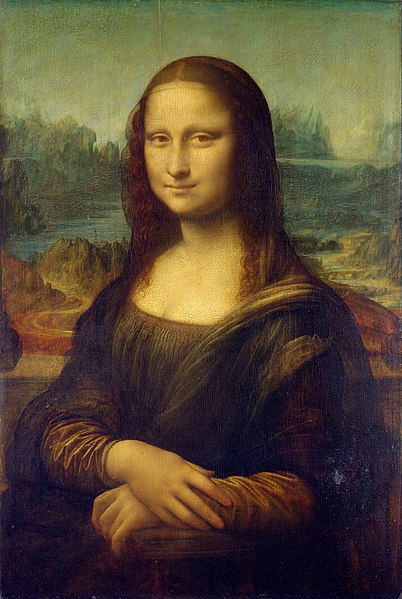
\includegraphics{monalisa}
	\caption[Sigils]{Some sigils\\
	\url{https://media.urbit.org/site/posts/essays/help-the-environment.jpg}}
	\labfig{marginsigils}
\end{marginfigure}

\section{Developing for Urbit}
\labsec{developing}

Urbit development can be divided into three cases:

\begin{enumerate}
	\item  Kernel development
	\item  Userspace development, Urbit-side (\gall~and generators)
	\item  Userspace development, client-side (Urbit API)
\end{enumerate}

This guide focuses on getting the reader up to speed on the second development case early, then branches out.

We encourage the reader to approach each example and exercise in the following spirit:

\begin{enumerate}
  \item  Identify the input and outputs, preferably at the data type level and contents.
	\item  Reason analogically from other Hoon examples available in the text and elsewhere.
	\item  Create and complete an outline of the code content.
	\item  Devise and compose a suitable test suite.
\end{enumerate}


\pagelayout{wide} % No margins
\addpart{Language Essentials}
\pagelayout{margin} % Restore margins

\setchapterpreamble[u]{\margintoc}
\chapter{Nock, A Combinator Language}
\labch{nock}


\section{Primitive rules and the combinator calculus}
\labsec{primitive}


A combinator calculus is one way of writing primitive computational systems.  Combinatory logic allows one to eliminate the need for variables (unknown quantities like $x$) and thus deal exclusively (?) with pure functions.

one combinator calculus



To understand how Nock expressions produce nouns as pure stateless functions, we need to introduce the \emph{subject}.  The subject is somewhat analogous to a namespace in other programming languages; it encompasses the computational context and the arguments.  Another way to put it is that the subject \emph{is} the argument to the Nock formula:  not all of the subject may be used in evaluating the formula, but it is all present.


Nock is a crash-only language; that is, while it can emit events that are interpretable by the runtime as errors that can be handled, Nock itself fails when an invalid operation occurs.

Nock is a standard of behavior, not necessarily an actual machine.  (It is an actual machine, of course, as a fallback, but the point is that any Nock virtual machine should implement the same behavior.)  We like to think of this analogous to solving a matrix.  Formally, given an equation

$$
A \vec{x} = \vec{b}
$$

the solution should be obtained as

$$
A^{-1} A \vec{x} = A^{-1} \vec{b} \rightarrow \vec{x} = A^{-1} \vec{b}
$$

This is correct, but often computationally inefficient to achieve.  Therefore we use this behavior as a standard definition for $\vec{x}$, but may actually obtain $\vec{x}$ using other more efficient methods.  Keep this in mind with Nock:  one has to know the specification but doesn't have to follow suit to implement it this way (thus, jet-accelerated Nock, Section~\ref{jetting}).

\subsection{Nock 4K}

The current version of Nock, Nock 4K, consists of six primitive rules as well as a handful of compound adjuncts.  The primitive rules are conventionally written in an explanatory pseudocode:

\begin{lstlisting}[style=nonumbers]
*[a 0 b]            /[b a]
*[a 1 b]            b
*[a 2 b c]          *[*[a b] *[a c]]
*[a 3 b]            ?*[a b]
*[a 4 b]            +*[a b]
*[a 5 b c]          =[*[a b] *[a c]]
\end{lstlisting}

with the following operations:

\begin{itemize}
  \item  \texttt{*} is the \emph{evaluate} operator, which operates on a cell of \texttt{[subject formula]};
  \item  \texttt{/} is the \emph{slot} operator or address \texttt{b} of [tree] \texttt{a};
  \item  \texttt{?} is the \emph{cell} operator, testing whether its operand is a cell.
  \item  \texttt{+} is the \emph{increment} operator.
  \item  \texttt{=} is the \emph{equality} operator, checking for structural equality of the operands evaluated against the subject \texttt{a}.
\end{itemize}

It is also instructive to write these as mathematical rules:

\begin{alignat*}{3}
*_{0}&[a](b) &&:= a_{b} \\
*_{1}&[a](b) &&:= b \\
*_{2}&[a](b,c) &&:= *({*[a](b)}, {*[a](c)}) \\
*_{3}&[a](b) &&:= \left\{\begin{matrix} \textrm{true} & \text{if cell} \\ \textrm{false} & \text{if atom} \end{matrix} \right. \\
*_{4}&[a](b) &&:= {*(a,b) + 1} \\
*_{5}&[a](b,c) &&:= ({*(a,b)} \stackrel{?}{=} {*(a,c)})
\end{alignat*}

where $*$ is the generic evaluate operator.  Furthermore, \textrm{true} is the integer $0$ while \textrm{false} is the integer $1$.
Each rule is referred to by its number; \eg~"Nock 3" refers to the cell test rule.

Nock operates on unsigned integers, with zero $0$ expressing the null or empty value.  Frequently this is written as a tilde, $\textasciitilde$ or \nullchr.  This value plays a complex role similar to \texttt{NULL} and \texttt{'\textbackslash 0'} in C and other programming languages—although, critically, it is still numeric.

%-------------------------------------------------------------------------------
\subsubsection[Nock 0]{Nock 0, Addressing}
\labsec{nock0}

\begin{lstlisting}[style=nonumbers]
*[a 0 b]            /[b a]
\end{lstlisting}

$$
*_{0}(a,b) := a_{b}
$$

Nock Zero allows the retrieval of nouns against the Nock subject.  Data access requires knowing the address and how to retrieve the corresponding value at that address.  The slot operator expresses this relationship using \texttt{a} as the subject and the atom \texttt{b} as the one-indexed address.

Every structure in Nock is a binary tree.  Elements are enumerated left-to-right starting at $1$ for the entire tree.


One common convention is to store values at the leftward leaves of rightward branches; this produces a cascade of values at addresses $2^{n}-2$.

\marginnote[2mm]{The address of a value in the Nock binary tree has no direct correspondence to its address in physical memory.  This latter is handled by the Nock runtime, avoiding the use of pointers in Nock code.}




By hand,


\marginnote[2mm]{
\dottar~implements Nock Two, which is of course \emph{evaluate}.
}

In the Dojo, you may evaluate this statement using the \pdottar~rune:

\begin{lstlisting}[style=nonumbers]
.*(TODO)
\end{lstlisting}

You may also use \texttt{++mock}

virtualization arm computes a formula.  `++mock` is Nock in Nock, however, so it is not very fast or efficient.

`++mock` returns a tagged cell, which indicates the kinds of things that can go awry:

- `%0` indicates success
- `%1` indicates a blocked calculation
- `%2` indicates a crash with stack trace

`++mock` is used in Gall and Hoon to virtualize Nock calculations and intercept scrys.  It is also used in Aqua, the testnet infrastructure of virtual ships.

%-------------------------------------------------------------------------------
\subsubsection[Nock 1]{Nock 1, Constant Reduction}
\labsec{nock1}

\begin{lstlisting}[style=nonumbers]
*[a 1 b]            b
\end{lstlisting}

$$
*_{1}(a,b) := b
$$

Nock One simply returns the constant value of noun \texttt{b}.

%-------------------------------------------------------------------------------
\subsubsection[Nock 2]{Nock 2, Evaluate}
\labsec{nock2}

\begin{lstlisting}[style=nonumbers]
*[a 2 b c]          *[*[a b] *[a c]]
\end{lstlisting}

$$
*_{2}[a](b,c) := *({*[a](b)}, {*[a](c)})
$$

%-------------------------------------------------------------------------------
\subsubsection[Nock 3]{Nock 3, Test Cell}
\labsec{nock3}

\marginnote[2mm]{
  Although unusual, Nock is by no means the only language to adopt $0$ as the standard of truth.  The POSIX-compliant shells such as Bash adopt the convention that $0$ is \texttt{TRUE}.  So do Ruby and Scheme, although with caveats.
}

Nock Three
zero as true (because there is one way to be right and many ways to be wrong).
loobean

%-------------------------------------------------------------------------------
\subsubsection[Nock 4]{Nock 4, Increment}
\labsec{nock4}
%-------------------------------------------------------------------------------
\subsubsection[Nock 5]{Nock 5, Test Equivalence}
\labsec{nock5}

Let us examine some Nock samples by hand and see if we can reconstruct what they do.  We will then create some new short programs and apply them by hand via the Nock rules.


\section{Compound rules}
\labsec{compound}

For the convenience of programmers working directly with Nock (largely the implementers of Hoon), a number of compound rules were defined that reduce to the primitive rules.  These implement slightly higher-order conventions such as a decision operator.  Each of these provide syntactic sugar that render Nock manipulations slightly less cumbersome.

\begin{lstlisting}[style=nonumbers]
*[a 6 b c d]        *[a *[[c d] 0 *[[2 3] 0 *[a 4 4 b]]]]
*[a 7 b c]          *[*[a b] c]
*[a 8 b c]          *[[*[a b] a] c]
*[a 9 b c]          *[*[a c] 2 [0 1] 0 b]
*[a 10 [b c] d]     #[b *[a c] *[a d]]

*[a 11 [b c] d]     *[[*[a c] *[a d]] 0 3]
*[a 11 b c]         *[a c]
\end{lstlisting}

with the following operation:

\begin{itemize}
  \item  \texttt{\#} is the \emph{replace} operator, which edits a noun by replacing part of it with another piece.
\end{itemize}

As mathematical rules, these would be:

\begin{alignat*}{3}
*_{6}&[a](b,c,d) &&:= \left\{ \begin{matrix} *[a](c) & \textrm{if } b \\ *[a](d) & \textrm{otherwise} \end{matrix} \right. \\
*_{7}&[a](b,c) &&:= *[*[a](b)](c) \\
*_{8}&[a](b,c) &&:= *[*[*[a](b)](a)](c) \\  %TODO CHECKME
*_{9}&[a](b,c) &&:= \left\{\begin{matrix} 0 & \text{if cell} \\ 1 & \text{if atom} \end{matrix} \right. \\
*_{10}&[a](b,c,d) &&:= {*(a,b) + 1} \\
*_{11}&[a](b,c,d) &&:= ({*(a,b)} \stackrel{?}{=} {*(a,c)}) \\
*_{11}&[a](b,c) &&:= ({*(a,b)} \stackrel{?}{=} {*(a,c)})
\end{alignat*}

where $*$ is the generic evaluate operator.

%-------------------------------------------------------------------------------
\subsubsection[Nock 6]{Nock 6, Conditional Branch}
\labsec{nock6}
%-------------------------------------------------------------------------------
\subsubsection[Nock 7]{Nock 7, Compose}
\labsec{nock7}
%-------------------------------------------------------------------------------
\subsubsection[Nock 8]{Nock 8, Declare Variable}
\labsec{nock8}
%-------------------------------------------------------------------------------
\subsubsection[Nock 9]{Nock 9, Produce Arm of Core}
\labsec{nock9}
%-------------------------------------------------------------------------------
\subsubsection[Nock 10]{Nock 10, Replace}
\labsec{nock10}
%-------------------------------------------------------------------------------
\subsubsection[Nock 11]{Nock 11, Hint to Interpreter}
\labsec{nock11}

\marginnote[2mm]{
There's also a "fake Nock" Rule Twelve, \pdotket, which exposes a namespace into Arvo.  More details on this follow in Section~\ref{TODO}.
}

With Nock under your belt, many of the quirks of Hoon become more legible.  For instance, since everything in Nock is a binary tree, so also everything in Hoon.  Nock also naturally gives rise to cores, which are a way of pairing operations and data in a cell.

Although Nock is the runtime language of Urbit, developers write actual code using Hoon.  Given a Hoon expression, you can produce the equivalent Nock formula using \pzaptis.

After this chapter, you may never write Nock code again.  That's fine!  We need to understand Nock to understand Hoon, but will not need to compose in Nock directly to do any work in Urbit, even low-level work.  (There is no \texttt{inline}~equivalent.)

\begin{lstlisting}[style=nonumbers]
> !=(+(1))
[4 1 1]

> !=((add 1 1))
[8 [9 36 0 1.023] 9 2 10 [6 [7 [0 3] 1 1] 7 [0 3] 1 1] 0 2]
\end{lstlisting}

(Why do these differ so much?  \texttt{++add} is doing a bit more than just adding a raw $1$ to an unsigned integer.  We'll walk through this function later in Section~TODO.)


One last piece is necessary for us to effectively interpret Nock code:  the implicit cons.  Cons is a Lisp function to construct a pair, or what in Nock terms we call a cell.  Many times we find Nock expressions in which the operand is a cell, and so TODO

\subsection{Nock Examples}

We will work through several Nock programs by hand.  Since each Nock program is a pure function and emits no side effects, when we have applied all of the rules to achieve a final value, we are done calculating the expression.

Infamously, Nock does not have a native decrement operator, only an increment (Rule Four).  Let us dissect a simple decrement operation in Nock:

\begin{lstlisting}[style=nonumbers]
> !=(|=(a=@ =+(b=0 |-(?:(=(a +(b)) b $(b +(b)))))))
[ 8
  [1 0]
  [1 8 [1 0] 8 [1 6 [5 [0 30] 4 0 6] [0 6] 9 2 10 [6 4 0 6] 0 1] 9 2 0 1]
  0
  1
]
\end{lstlisting}

which can be restated in one line as

\begin{lstlisting}[style=nonumbers]
[8 [[1 0] [1 8 [1 0] 8 [1 6 [5 [0 30] 4 0 6] [0 6] 9 2 10 [6 4 0 6] 0 1] 9 2 0 1] 0 1]]
\end{lstlisting}

or in many lines as

\begin{lstlisting}[style=numbers]
[8
  [1 0]
  [1 [8
       [1 0]
       [8
         [1 [6
              [5
                [0 30]
                [4 0 6]
              ]
              [0 6]
              [9
                2
                [10
                  [6 4 0 6]
                  [0 1]
                ]
              ]
            ]
           [9 2 0 1]
         ]
       ]
     ]
  ]
  [0 1]
]
\end{lstlisting}

(It's advantageous to see both.)

We can pattern-match a bit to figure out what the pieces of the Nock are supposed to be in higher-level Hoon.  From the Hoon, we can expect to see a few kinds of structures:  a trap, a test, a `sample`.  At a glance, we seem to see Rules One, Five, Six, Eight, and Nine being used.  Let's dig in.

(Do you see all those `0 6` pieces?  Rule Zero means to grab a value from an address, and what's at address `6`?  The `sample`, we'll need that frequently.)

The outermost rule is Rule Eight `*[a 8 b c]→*[[*[a b] a] c]` computed against an unknown subject (because this is a gate).  It has two children, the `b` `[0 1]` and the `c` which is much longer.  Rule Eight is a sugar formula which essentially says, run `*[a b]` and then make that the head of a new subject, then compute `c` against that new subject.  `[0 1]` grabs the first argument of the `sample` in the `payload`, which is represented in Hoon by `a=@`.

The main formula is then the body of the gate.  It's another Rule Eight, this time to calculate the `b=0` line of the Hoon.

There's a Rule One, or constant reduction to return the bare value resulting from the formula.

Then one more Rule Eight (the last one!).  This one creates the default subject for the trap \texttt{\$}; this is implicit in Hoon.

Next, a Rule Six.  This is an `if`/`then`/`else` clause, so we expect a test and two branches.

- The test is calculated with Rule Five, an equality test between the address `30` of the subject and the increment of the `sample`.  In Hoon, `=(a +(b))`.

- The \texttt{[0 6]} returns the `sample` address.

- The other branch is a Rule Nine reboot of the subject via Rule Ten.  Note the `[4 0 6]` increment of the `sample`.

Finally, Rule Nine is invoked with `[9 2 0 1]`, which grabs a particular arm of the subject and executes it.

Contrast the built-in `++dec` arm:

\begin{lstlisting}
> !=((dec 1))
[8 [9 2.398 0 1.023] 9 2 10 [6 7 [0 3] 1 1] 0 2]
\end{lstlisting}

for which the Hoon is:


\begin{lstlisting}
++  dec
  |=  a=@
  ?<  =(0 a)
  =+  b=0
  |-  ^-  @
  ?:  =(a +(b))  b
  $(b +(b))
\end{lstlisting}

Scan for pieces you recognize:  the beginning of a cell is frequently the rule being applied.

In tall form,

\begin{lstlisting}
[8
  [9
    [2.398 [0 1.023]]
  ]
  [9 2
       [10
         [6 7 [0 3] 1 1]
         [0 2]
       ]
  ]
]
\end{lstlisting}

What's going on with the above \texttt{++dec} is that the Arvo-shaped subject is being addressed into at `2.398`, then some internal Rule Nine/Ten/Six/Seven processing happens.

\section{Kelvin versioning}
\labsec{kelvin}

Each version of Nock

telescopic versioning

\section{Exercises}

Compose a Nock interpreter in a language of your choice.  (These aren't full Arvo interpreters, of course, since you don't have the Hoon, \zuse, and vane subject present.)

\setchapterpreamble[u]{\margintoc}
\chapter{Elements of Hoon}
\labch{hoonelemens}


\section{Reading the Runes}
\labsec{he:reading}

\subsection{Objectives}
\labsec{he:objectives}

The goals of this chapter are for you to be able to:

\begin{enumerate}
  \item  Identify Hoon runes and children in both inline and long-form syntax.
  \item  Trace a short Hoon expression to its final result.
  \item  Execute Hoon code within a running ship.
  \item  Produce output as a side effect using the \sigpam~rune.
\end{enumerate}

\marginnote[2mm]{
Although not a compiled language, the binary-tree structure of Hoon can lead to fairly involved programs which are difficult to type and parse as directly as some other languages afford.  We instead encourage you to use one of three methods to run Hoon programs:

\begin{enumerate}
  \item  The Dojo REPL, which offers some convenient shortcuts to modify the subject for subsequent commands.
  \item  A tight loop of text editor and running fakezod.
  \item  The online interactive sandbox at \url{https://approaching-urbit.com}{\texttt{approaching-urbit.com}}
\end{enumerate}
}

For the first several exercises, we will suggest that you utilize one of these methods in particular so that you get a feel for how each works.  After you are more comfortable working with Hoon code on Urbit, we will refrain.


The terminology used is often unfamiliar.  Sometimes this means that you are dealing with a truly new concept (and overloading an older word like "subroutine" or "function" would obfuscate), and sometimes you are dealing with an internal aspect that doesn't really map well to other systems.  The strangeness can be frustrating.  The strangeness can make concepts fresh again.  You'll encounter both as you move ahead.

Each rune accepts at least one child, except for \pzapzap~(crash).  Most runes accept a definite number of children, but a few can accept a variable number; these use \tistis~or \hephep~digraphs to indicate termination of the running series.

\section{Irregular Forms}
\labsec{irregular}

Many runes in common currency are not written in their regular form (tall or wide), but rather using syntactic sugar as irregular.

For instance, \pcenhep~is most frequently written using parentheses \texttt{()} which permits a Lisp-like calling syntax:

\begin{lstlisting}[language=hoon,
                   style=nonumbers]
(add 1 2)
\end{lstlisting}

is equivalent to

\begin{lstlisting}[language=hoon,
                   style=nonumbers]
%-  add  [1 2]
\end{lstlisting}

which in turn is also equivalent to

\begin{lstlisting}[language=hoon,
                   style=nonumbers]
%-(add [1 2])
\end{lstlisting}

Developers balance expressiveness, comprehensibility, and pattern-matching in deciding how lapidary to compose a runic expression.  Many extremely common patterns were soon subsumed by a sugar rune.

Hoon parses to an abstract syntax tree (AST), which includes cleaning up all of the sugar syntax and non-primitive runes.  To see the AST of any given Hoon expression, use \pzapcom.

\marginnote[2mm]{
While parsing this AST is beyond the text at this point, note significant features like \texttt{\%tsfs} for \tisfas~and \texttt{\%sand} for aura-castable values.
}
\begin{lstlisting}[language=hoon,
                   style=nonumbers]
> !,(*hoon =/(n 4 +(n)))
[%tsfs p=term=%n q=[%sand p=%ud q=4] r=[%dtls p=[%wing p=~[%n]]]]
\end{lstlisting}


\section{Nouns}
\labsec{nouns}

All values in Urbit are nouns, meaning either atoms or cells.  An atom is an unsigned integer.  A cell is a pair of nouns.  Since all values are ultimately integers, we need a way to tell different "kinds" (or applications) of integers apart.  Enter auras.

\subsection{Atoms}
\labsec{atoms}

\marginnote[2mm]{
For what it may be worth, having all integers isn't that different from any other digital machine, built on binary numbers.  These all derive ultimately from \href{https://en.wikipedia.org/wiki/Gödel_numbering}{Gödel numbering} as introduced by Gödel in the proof of his famous incompleteness theorems.  Urbit makes this about as apparent as C does (via \texttt{union}, for instance), but it's first-order accessible via the Dojo REPL.
}
Atoms have auras which are tagged types.  In other words, an aura is a bit of metadata Hoon attaches to a value which tells Urbit how you intend to use a number.  (Of course, ultimately an aura is itself an integer as well!)  The default aura for a value is \patud, unsigned decimal, but of course there are many more.  Aura operations are extremely convenient for converting between representations.  They are also used to enforce type constraints on atoms in expressions and gates.

For instance, to a machine there is no fundamental difference between binary $\ub 1101\,1001$, decimal $217$, and hexadecimal $\ux d9$.  A human coder recognizes them as different encoding schemes and associates tacit information with each:  an assembler instruction, an integer value, a memory address.  Hoon offers two ways of designating values with auras:  either directly by the formatting of the number (such as \texttt{0b1101.1001}) or using the irregular syntax \texttt{`@`}:

\begin{lstlisting}[language=hoon,
                   style=nonumbers]
0b1101.1001
`@ud`0b1101.1001  :: yields 217
`@ux`0b1101.1001  :: yields 0xd9
\end{lstlisting}

\begin{example}
Try the following auras.  See if you can figure out how each one is behaving.

\begin{lstlisting}[language=hoon]
`@ud`0x1001.1111
`@ub`0x1001.1111
`@ux`0x1001.1111
`@p`0x1001.1111

`@ud`.1
`@ux`.1
`@ub`.1
`@sb`.1

`@p`0b1111.0000.1111.0000

`@ta`'hello'
`@ud`'hello'
`@ux`'hello'
`@uc`'hello'
`@sb`'hello'
`@rs`'hello'
\end{lstlisting}
\end{example}

\marginnote[2mm]{For a full table of auras, see Appendix~\ref{app:auras}.}
The atom/aura system represents all simple data types in Hoon:  dates, floating-point numbers, text strings, Bitcoin addresses, and so forth.  Each value is represented in least-significant byte (LSB) order; for instance, a text string may be deconstructed as follows:

\begin{tabular}{l}
  \texttt{'Urbit'} \\
  \texttt{0b111.0100.0110.1001.0110.0010.0111.0010.0101.0101} \\
  \texttt{0b111.0100} \texttt{0b110.1001} \texttt{0b110.0010} \\ \texttt{0b111.0010} \texttt{0b101.0101} \\
  $116\;105\;98\;114\;85$ (ASCII characters) \\
  t i b r U
\end{tabular}

Note in the above that leading zeroes are always stripped.  Since each atom is an integer, there is no way to distinguish $0$ from $00$ from $000$ etc.

In this vein, it's worth mentioning that Dojo automatically parses any typed input and disallows invalid representations.  This can lead to confusion until you are accustomed to the type signatures; for instance, try to type \texttt{0b0001} into Dojo.

\paragraph{Operators}.  Hoon has no primitive operators.  Instead, aura-specific functions or \emph{gates} are used to evaluate one or more atoms to produce basic arithmetic results.  Gate names are conventionally prefixed with \texttt{++} which designates them as \emph{arms} of a \emph{core}.  (More on this terminology in Section~\ref{TODO}.)  Some gates operate on any input atom auras, while others enforce strict requirements on the types they will accept.  Gates are commonly invoked using a Lisp-like syntax and a reverse-Polish notation (RPN), with the operator first followed by the first and second (and following) operands.

\begin{tabular}{lll}
  Operation & Function & Example \\ \hline \\
  Addition & \texttt{++add} & \texttt{(add 1 2)} $\rightarrow$ \texttt{3} \\
  Subtraction & \texttt{++sub} & \texttt{(sub 4 3)} $\rightarrow$ \texttt{1} \\
  Multiplication & \texttt{++mul} & \texttt{(mul 5 6)} $\rightarrow$ \texttt{30} \\
  Division & \texttt{++div} & \texttt{(div 8 2)} $\rightarrow$ \texttt{4} \\
  Modulus/Remainder & \texttt{++mod} & \texttt{(mod 12 7)} $\rightarrow$ \texttt{5} \\
\end{tabular}

Following Nock's lead, Hoon uses loobeans ($0$ = $\textrm{true}$) rather than booleans for logical operations.  Loobeans are written \yes~for $\textrm{true}$, $0$, and \no~for $\textrm{false}$, $1$.

\begin{tabular}{lll}
  Operation & Function & Example \\ \hline \\
  Greater than, $>$ & \texttt{++gth} & \texttt{(gth 5 6)} $\rightarrow$ \no \\
  Greater than or equal to, $\geq$ & \texttt{++gte} & \texttt{(gte 5 6)} $\rightarrow$ \no \\
  Less than, $<$ & \texttt{++lth} & \texttt{(lth 5 6)} $\rightarrow$ \yes \\
  Less than or equal to, $\leq$ & \texttt{++lte} & \texttt{(lte 5 6)} $\rightarrow$ \yes \\
  Equals, $=$ & \texttt{=} & \texttt{=(5 5)} $\rightarrow$ \yes \\
  Logical \texttt{AND}, $\land$ & \texttt{\&} & \texttt{\&(\%.y \%.n)} $\rightarrow$ \no \\
  Logical \texttt{OR}, $\lor$ & \texttt{|} & \texttt{|(\%.y \%.n)} $\rightarrow$ \yes \\
  Logical \texttt{NOT}, $\neg$ & \texttt{!} & \texttt{!\%.y} $\rightarrow$ \no \\
\end{tabular}

Since all operations are explicitly invoked Lisp-style within nested parentheses, there is no need for explicit operator precedence rules.

$$
(a < b) \land ((b \geq c) \lor d)
$$

\begin{lstlisting}[language=hoon,
                   style=nonumbers]
\&((lth a b) (|((gte b c) d)))
\end{lstlisting}

The Hoon standard library, largely in \zuse, further defines bitwise operations, arithmetic for both integers and floating-point values (half-width, single-precision, double-precision, and quadruple-precision), string operations, and more.  These are introduced incidentally as necessary and listed in more detail in Appendix~\ref{stdlib}.

\subsection{Cells}
\labsec{cells}

Just as all structures in Nock are binary trees, so too with Hoon.  This can occasionally lead to some awkward addressing when composing tetchy library code segments that need to interface with many different kinds of gates, but by and large is an extremely helpful discipline of thought.


binary tree format
flattened representation/convention

\marginnote[2mm]{Binary trees are explained in more detail in Section~\ref{nock0}.}

Hoon values are addressed as elements in a binary tree.


Finally, the most general mold is \texttt{*} which simply matches any noun—and thus anything in Hoon at all.

\section{Hoon as Nock Macro}
\labsec{macro}

The point of employing Hoon is, of course, that Hoon compiles to Nock.  Rather than even say \emph{compile}, however, we should really just say Hoon is a \emph{macro} of Nock.  Each Hoon rune, data structure, and effect corresponds to a well-defined Nock primitive form.  We may say that Hoon is to Nock as C is to assembler, except that the Hoon-to-Nock transformation is completely specified and portable.  Hoon is ultimately defined in terms of Nock; many Hoon runes are defined in terms of other more fundamental Hoon runes, but all runes parse unambiguously to Nock expressions.


Hoon expands on Nock primarily through the introduction of metadata


Each Hoon rune has an unambiguous mapping to a Nock representation.  Furthermore, each rune has a well-defined binary tree structure and produces a similarly well-structured abstract syntax tree (AST).  As we systematically introduce runes, we will expand on what this means in each case:  for now, let's examine two runes without regard for their role.

\begin{enumerate}
  \item  \pbartis~produces a \emph{gate} or function.  Every gate has the same shape, which means certain assumptions about data access and availability can be made.

    \begin{lstlisting}[language=hoon,
                       style=nonumbers]
::  XOR two binary atoms
|=  [a=@ub b=@ub]
`@ub`(mix a b)
    \end{lstlisting}

    maps to the Nock code

    \begin{lstlisting}[language=hoon,
                       style=nonumbers]
[8 [1 0 0] [1 8 [9 1.494 0 4.095] 9 2 10 [6 [0 28] 0 29] 0 2] 0 1]
    \end{lstlisting}

    This Nock code is fully annotated in Example~\ref{ex:nock:xor}.

  \item  TODO
\end{enumerate}


We call Hoon's data type specifications \emph{molds}.  Molds are more general than atoms and cells, but these form particular cases.  Hoon uses molds as a way of matching Nock tree structures (including Hoon metadata tags such as auras).

\section{Subject-Oriented Programming}

TODO
arms legs basics

\marginnote[2mm]{
Be careful to not confuse \irrtis, which evaluates to \dottis, with the various \wut~runes like \wuttis.
}

\section{Key Data Structures}
\labsec{he:structures}

\subsection{Lists}
\labsec{he:lists}


Lests

\subsection{Text}
\labsec{text}

\marginnote[2mm]{Both cords and tapes are casually referred to as strings.}

Hoon recognizes two basic text types:  the \emph{cord} or \patt~and the \emph{tape}.  Cords are single atoms containing the text as UTF-8 bytes interpreted as a single stacked number.  Tapes are lists of individual one-element cords.

\marginnote[2mm]{Lists are null-terminated, and thus so are tapes.}

Cords are useful as a compact primary storage and data transfer format, but frequently parsing and processing involves converting the text into tape format.  There are more utilities for handling tapes, as they are already broken up in a legible manner.

\begin{lstlisting}[language=hoon,
                   style=nonumbers]
++  trip
  |=  a=@  ^-  tape
  ?:  =(0 (met 3 a))  ~
  [^-(@ta (end 3 1 a)) $(a (rsh 3 1 a))]
\end{lstlisting}


For instance, \texttt{trip} converts a cord to a tape; \texttt{crip} does the opposite.

%\marginnote[2mm]{
%\begin{lstlisting}
%++  trip
%  |=  a/@  ^-  tape
%  ?:  =(0 (met 3 a))  ~
%  [^-(@ta (end 3 1 a)) $(a (rsh 3 1 a))]
%\end{lstlisting}
%\texttt{++met}, \texttt{++end}, and \texttt{++rsh} are bitwise manipulation gates.
%}

\marginnote[2mm]{
%\begin{lstlisting}
\texttt{++  crip  |=(a=tape `@t`(rap 3 a))}
%\end{lstlisting}

\texttt{++rap} assembles the list interpreted as cords with block size of $2^3$ (in this case).
}


All text in Urbit is UTF-8 (and typically just 8-bit ASCII).  The \patc~UTF-32 aura is only used by \dill and Hood (the Dojo terminal agent).


\subsection{Cores and Derived Structures}
\labsec{he:cores-derived}

\subsubsection{Cores}
\labsec{he:core}

The core is the primary nontrivial data structure of Nock:  atoms, cells, cores.  A core is defined as a cell of \texttt{battery payload}; in the abstract this simply divides the \texttt{battery} or code from the \texttt{payload} or data.  Cores can be thought of as similar to objects in object-oriented programming languages, but possess a completely standard structure which allows for detailed introspection and “hot-swapping” of core elements.  Everything in standard Hoon and Arvo that cannot be reduced to an atom or a cell is \emph{de facto} a core.  (Indeed, if one wished to separate code and data in a structure, the only other logical choice one would have available is to flip the order of battery and payload.)

Conventionally, most cores are either produced by the \pbarcen~rune or are instances of a more complex form (such as a door).  Cores are a “live” type; they are not simply holders of data but are expected to operate on data, just as it is uncommon to see a C++ object which only holds data.  (The role of a C \texttt{struct} is approximated by the \buccen~tagged union.)

Some terminology is in order, to be expanded on subsequently.  An \emph{arm} is a Hoon expression to be evaluated against the
arms
legs
Arms and legs are both \emph{limbs}.  (These must be distinguished from \emph{wings}, which are resolution paths pointing to a limb.)


\subsubsection{Traps}
\labsec{he:trap}

The trap creates the basic looping mechanism in Hoon, a special instance of a core which is capable of concisely recursing into itself.  The trap is formally a core with one arm named \buc, and it is either created with \pbarhep~(for instant evaluation) or \pbardot~(for deferred evaluation).

In practice, traps are used almost exclusively as recursion points, much like loops in an imperative language.  For instance, the following program counts from 5 down to 1, emitting output via \psigpam~at each iteration, then return \sig.

\begin{lstlisting}[language=hoon,
                   style=nonumbers]
=/  count  5
|-
  ?:  =(count 0)  ~
~&  count
$(count (dec count))
\end{lstlisting}

\marginnote[2mm]{
The \texttt{\$()} notation is shorthand for \pcentis, which evaluates a wing given a set of changes.
}
The final line \texttt{\$(count (dec count))} serves to modify the subject (at \texttt{count}) then to pull the \buc~arm again.  In practice the tree unrolls as follows, with indentation indicating code running “inside” of another rune.

\begin{lstlisting}[language=hoon,
                   style=nonumbers]
=/  count  5
|-
  ?:  =(count 0)  ~
  ~&  count
  =/  count  (dec count)
  ?:  =(count 0)
  TODO think about how to unroll this in a visually pleasing manner that isn't
  a total lie
$(count (dec count))
\end{lstlisting}


recursive


\subsubsection{Gates}
\labsec{he:gate}

Similar to how a trap is a core with one arm, a gate is a core with one arm and a sample.  This means that new per-invocation data are available in the gate's subject.


A gate can recurse into itself like a trap when necessary.  In this example, the gate accepts a value \texttt{n} (the gate's \texttt{spec}) and applies an arm (implicitly named \buc) which carries out the calculation.  (Say it with me:  \texttt{sample}/\texttt{payload}.)  When the \texttt{\$()} recursion point is reached, the entire \buc~arm is re-evaluated with the specified change of $\texttt{n} \rightarrow \texttt{n} - 1$.

\begin{lstlisting}[language=hoon,
                   caption={Calculating a factorial using recursion.  (Example from Tlon documentation.)}]
|=  n=@ud             :: accept a single value n for n!
?:  =(n 1)  1         :: check n ≟ 1; if so, return 1
(mul n $(n (dec n)))  :: multiply n times the product of this arm w/ n-1
\end{lstlisting}

That is, when one reads this program, one reads it falling into two components:

\begin{lstlisting}[language=hoon,
                   style=nonumbers]
|=  n=@ud             :: accept a single value n for n!
?:  =(n 1)  1         :: check n ≟ 1; if so, return 1
(mul n $(n (dec n)))  :: multiply n times the product of this arm w/ n-1
\end{lstlisting}



\subsubsection{Doors}
\labsec{he:door}

\barcab

The \pbarcen~rune produces a dry core, thus all arms it contains are dry.

The \pbarpat~rune produces a wet core, so it can contain wet arms.

Doors are superficially similar to gates, but calling an arm in a door is more general:  the calling convention for a gate replaces the sample then pulls the \buc~arm, while the calling convention for a door replaces the sample then pulls whichever arm has been requested.

Since \dot~refers to the subject TODO:expand, this yields the ability to manipulate the sample without calling any arm directly.  The following examples illustrate:

\begin{lstlisting}[language=hoon,
                   style=nonumbers]
> (add [1 5]})              :: call a gate
6
> ~($ add [1 5])            :: call the $ arm in the door
6
> ~(. add [1 5])            :: update the sample (arguments) but don't evaluate
<1.otf [[@ud @ud] <45.xig 1.pnw %140>]>
> =<  $  ~(. add [1 5])     :: call the $ arm of the door with updated sample
6
> =/  addd  ~(. add [1 5])  :: do the same thing but in two steps
  =<  $  addd
6
\end{lstlisting}


At this point, we need to step back and contextualize the power afforded by the use of cores.  In another language, such as C or Python, we specify a behavior but have relatively little insight into the instantiation effected by the compiler:

\begin{lstlisting}[language=python,
                   caption={Python loop to sum the length of several strings.}]
metals = ['gold', 'iron', 'lead', 'zinc']
total = 0
for metal in metals:
    total = total + len(metal)
\end{lstlisting}

\begin{lstlisting}[language=jvmis,
                   caption={Python bytecode equivalent}]
1          0 LOAD_CONST               0 ('gold')
           2 LOAD_CONST               1 ('iron')
           4 LOAD_CONST               2 ('lead')
           6 LOAD_CONST               3 ('zinc')
           8 BUILD_LIST               4
          10 STORE_NAME               0 (metals)

2         12 LOAD_CONST               4 (0)
          14 STORE_NAME               1 (total)

3         16 LOAD_NAME                0 (metals)
          18 GET_ITER
     >>   20 FOR_ITER                16 (to 38)
          22 STORE_NAME               2 (metal)

4         24 LOAD_NAME                1 (total)
          26 LOAD_NAME                3 (len)
          28 LOAD_NAME                2 (metal)
          30 CALL_FUNCTION            1
          32 BINARY_ADD
          34 STORE_NAME               1 (total)
          36 JUMP_ABSOLUTE           20
     >>   38 LOAD_CONST               5 (None)
          40 RETURN_VALUE
\end{lstlisting}

Many popular programming languages specify \emph{behavior} rather than \emph{implementation}.  By specifying Hoon as a macro language over Nock, the Urbit developers collapse this distinction.

For Hoon (like Lisp), the structure of execution is always front-and-center, or at least only thinly disguised.  When one creates a core with a given behavior, one can immediately envision the shape of the underlying Nock.  This affords one immense power to craft efficient, effective, graceful programs.

\begin{lstlisting}[language=hoon,
                   caption={Hoon trap to sum the length of several tapes.}]
=/  metals  `(list tape)`~["gold" "iron" "lead" "zinc"]
=/  count  0
=/  total  0
|-
  ?:  =(count (lent metals))  total
  =/  metal  `tape`(snag count metals)
$(total (add total (lent metal)), count +(count))
\end{lstlisting}

\begin{lstlisting}[language=hoon,
                   caption={Nock equivalent}]
\end{lstlisting}

\subsection{Molds}
\labsec{he:molds}



Most software programs require—or at least are greatly simplified by—custom type definitions.  These are customarily defined with a \barcen~core preceding the \barcab~door definition.  We commonly see three runes supporting this structure:

\begin{itemize}
  \item  \lusbuc~creates a type constructor arm to define and validate type definitions.
  \item  \buccen~creates a collection of named values (type members).
  \item  \bucwut~defines a union, a set validating membership across a defined collection of items.
\end{itemize}

%TODO one without type union, then one with

To illustrate these, we serially consider several ways to define a vehicle.  In the first, we employ only \lusbuc~to capture key vehicle characteristics.  Using only \lusbuc, it's hard to say much of interest:

\begin{lstlisting}[style=nonumbers]
+$  vehicle  tape               :: vehicle identification number
\end{lstlisting}

By permitting collections of named type values with \buccen, we can produce more complicated structures:

\begin{lstlisting}[style=nonumbers]
+$  vehicle
  $%  vin=tape                  :: vehicle identification number
      owner=tape                :: car owner's name
      license=tape              :: license plate
  ==
\end{lstlisting}

Type definition arms can rely on other type definition arms available in the subject:

\begin{lstlisting}[style=nonumbers]
+$  vehicle
  $%  vin=tape                  :: vehicle identification number
      owner=tape                :: car owner's name
      license=tape              :: license plate
      kind=kind                 :: vehicle manufacture details
  ==
+$  kind
  $%  make=tape                 :: vehicle make
      model=tape                :: vehicle model
      year=@da                  :: nominal year of manufacture (use Jan 1)
  ==
\end{lstlisting}

\marginnote[2mm]{ \\ \\ \\ \\ \\ \\ \\ \\ \\ \\ \\ \\
In general, Hoon style does not require you to be careful about masking variable names in the subject.  Rarely, this introduces surprising bugs but is typically contextually apparent to the developer.
}
Finally, by introducing unions with \bucwut, a type definition arm can validate possible values:

\begin{lstlisting}[style=nonumbers]
+$  vehicle
  $%  vin=tape                  :: vehicle identification number
      owner=tape                :: car owner's name
      license=tape              :: license plate
      kind=kind                 :: vehicle manufacture details
  ==
+$  kind
  $%  make=tape                 :: vehicle make
      model=tape                :: vehicle model
      year=@da                  :: nominal year of manufacture (use Jan 1)
  ==
+$  make                        :: permitted vehicle makes
  ?(%acura %chrysler %delorean %dodge %jeep %tesla %toyota)
\end{lstlisting}


\subsection{Maps, Sets, Tree}
\labsec{macro}

units

\section{Generators}
\labsec{he:generators}

Generators are standalone Hoon expressions that evaluate and may produce side effects, as appropriate.  They are closely analogous to simple scripts in languages such as Bash or Python.  By using generators, one is able to develop more involved Hoon code and run it repeatedly without awkwardness.

\marginnote[2mm]{You may also see commands beginning with a \texttt{|}~symbol; these are Hood commands instead.}

To run a generator on a ship, prefix its name with \texttt{+}.  Arguments may be required or optional.

\begin{lstlisting}[style=nonumbers]
+moon TODO
\end{lstlisting}

\subsection{Running Developer Code on an Urbit Ship}
\labsec{he:running}

Since the Urbit file system, called \clay, is independent of the Unix file system on which it is hosted, you must commit your Unix-side code into your pier.

If we \texttt{cd} into the ship's pier in Unix and \texttt{ls} the directory contents, by default we see nothing.  With \texttt{ls -l}, a \texttt{.urb/} directory containing the ship's configuration and contents in obfuscated format becomes visible.  This directory is not interpretable by us now, so we leave it until a later discussion of the Urbit binary.  To move files into \clay, we must synchronize Urbit and Unix together.  We initiate this inside of the running ship; run the Urbit system command:

\begin{lstlisting}[style=nonumbers]
|mount %
\end{lstlisting}

where \texttt{\%} represents the current (home) path in \clay.  Unix-side, run \texttt{ls} again and a \texttt{home/} directory appears with a number of children:  \texttt{app/}, \texttt{gen/}, \texttt{lib/}, \texttt{mar/}, and so forth.  This is the internal esoteric structure of \clay~made manifest to Unix.

\marginnote[2mm]{\clay~implements several \emph{desks}, which are like branches in version control systems; the most important of these are \chome~and \ckids.}
Generally speaking, we compose \emph{generators}, which are short Hoon scripts.  These are created in or copied into the \texttt{home/mar/} directory, and then must be synchronized with Urbit's \clay.  Commit the change:

\begin{lstlisting}[style=nonumbers]
|commit %home
\end{lstlisting}

and the generator is now available within \clay.

\subsection{Naked Generators}
\labsec{he:naked}

As we start to compose generators,

A naked generator is so called because it contains no metadata for the Arvo interpreter.

\subsection{\say~generators}
\labsec{he:say}

\subsection{\ask~generators}
\labsec{he:ask}

\section{Libraries}
\labsec{libraries}

\section{Unit Tests}
\labsec{unittests}

\section{Building Code}
\labsec{building}

\section{Exercises}

The vertical direction presents a six-step process that prompts students to
read the problem statement, figure out the data that is needed to represent the information of interest, and illustrate their insight with concrete examples;

articulate a purpose statement that concisely describes what the function or program is supposed to compute, including a signature;

work through functional examples, that is, explain what the function or program is supposed to produce when given certain inputs, based on steps 1 and 2;

create an outline of the program, based on steps 1 and 2;

fill in the outline from step 4, using steps 2 and 3; and

turn the examples from step 2 into a test suite for the program from step 5.

\setchapterpreamble[u]{\margintoc}
\chapter{Advanced Hoon}
\labch{advancedhoon}


\section{Cores}
\labsec{cores}

\subsection{Variadicity}
\labsec{variadicity}

\subsection{Genericity}
\labsec{genericity}

\section{Molds}
\labsec{molds2}

\subsection{Polymorphism}
\labsec{polymorphism}

\section{Rune Families}
\labsec{runefamilies}

\section{Marks and Structures}
\labsec{marks}

\section{Helpful Tools}
\labsec{tools}

\section{Deep Dives}
\labsec{deepdives}

\subsection{Text Stream Parsing}
\labsec{text}

\subsection{JSON Parsing}
\labsec{json}

\subsection{HTML/XML Parsing}
\labsec{sail}


\pagelayout{wide} % No margins
\addpart{System Development}
\pagelayout{margin} % Restore margins

\setchapterpreamble[u]{\margintoc}
\chapter{The Kernel}
\labch{kr}

\section{Objectives}
\labsec{kr:objectives}

The goals of this chapter are for you to be able to:

\begin{enumerate}
  \item  Diagram the structure of Arvo as stateful event processor.
  \item  Follow a move trace to see how an event is processed by Arvo.
  \item  Enumerate the primary vanes of Arvo and their roles.
  \item  Scry into each vane for run-time information.
  \item  Query and manipulate ship keys from Azimuth and \jael.
\end{enumerate}


\section{Arvo}
\labsec{kr:arvo}

We could do worse than to start our exploration of the Urbit kernel than to quote the Whitepaper itself on the subject of Arvo:

\begin{quote}
The fundamental unit of the Urbit kernel is an event called a \texttt{+\$move}.  Arvo is primarily an event dispatcher between moves created by vanes.  Each move therefore has an address and other structured information.  (\cite{Yarvin2017})
\end{quote}

Every vane defines its own structured events (\texttt{+\$move}s).  Each unique kind of structured event has a unique, frequently whimsical, name.  This can make it challenging to get used to how a particular vane behaves.

\marginnote[2mm]{The system-level instrumentation of Arvo is described in Chapter~\ref{support}.}

Arvo is essentially an event handler which can coordinate and dispatch messages between vanes as well as emit \unix~events (side effects) to the underlying (presumed Unix-compatible) host OS.  Arvo as hosted OS does not carry out any tasks specific to the machine hardware, such as memory allocation, system thread management, and hardware- or firmware-level operations.  These are left to the \emph{king} and \emph{serf}, the daemon processes which together run Arvo.

Arvo is architected as a state machine, the deterministic end result of the event log.  We need to examine Arvo from two separate angles:

\begin{enumerate}
  \item  Event processing engine and state machine (vane coordinator)
  \item  Standard noun structure (“Arvo-shaped noun”)
\end{enumerate}

\subsection{Event Processing Engine}
\labsec{kr:arvo-state}

\begin{quote}
A vanilla event loop scales poorly in complexity.  A system event is the trigger for a cascade of internal events; each event can schedule any number of future events.  This easily degenerates into “event spaghetti.”  Arvo has “structured events”; it imposes a stack discipline on event causality, much like imposing subroutine structure on \texttt{goto}s.  (\cite{Yarvin2017})
\end{quote}

Arvo events are known as \texttt{++move}s, containing metadata and data.  Arvo recognizes four types of moves:

\begin{enumerate}
  \item  \pass~events are forward calls from one vane to another (or back to itself, occasionally), and
  \item  \give~events are returned values and move back along the calling duct.
  \item  \slip~events [TODO think of like ref counting?].  (\slip~events are common only in the initial system boot process or in over-the-air updates to Arvo.)
  \item  \unix~events communicate from Arvo to the underlying binary in such a way as to emit an external effect (an \ames~network communication, for instance, or text input and output).
\end{enumerate}

show structure of a card

"Each vane defines a protocol for interacting with other vanes (via Arvo) by defining four types of cards: tasks, gifts, notes, and signs."
"In other words, there are only four ways of seeing a move: (1) as a request seen by the caller, which is a note. (2) that same request as seen by the callee, a task. (3) the response to that first request as seen by the callee, a gift. (4) the response to the first request as seen by the caller, a sign."
(TODO move trace work here)

Without reference to the particular content of vanes, let us briefly diagram a “move trace”, or examination of how an event generated by a vane produces results via Arvo.

TODO remote call via \ames?

\begin{quote}
"An interrupted event never happened.  The computer is deterministic; an event is a transaction; the event log is a log of successful transactions. In a sense, replaying this log is not Turing complete. The log is an existence proof that every event within it terminates.  (\cite{Yarvin2017})
\end{quote}

\begin{example}{Tradecraft:  Tracing}
Now that we have discussed how Arvo processes events, we can turn our attention to how particular real events are actually processed.

Urbit supports tracing the behavior of each event using a command-line flag, conventionally \texttt{-j}.  Start an existing Urbit ship using

\begin{lstlisting}[language=bash,
                   style=nonumbers]
$ urbit -j sampel-palnet
\end{lstlisting}

Initiate an event:

\begin{lstlisting}[language=hoon,
                   style=nonumbers]
> (add 1 2)
\end{lstlisting}

Tracefiles will appear in \texttt{sampel-palnet/.urb/put/trace}.  Copy these JSON files to a working directory and open them using an appropriate utility.  There may be some lag in generating the tracefiles, and it requires discernment to locate the relevant move trace elements.

TODO
\end{example}

\begin{example}{Tradecraft:  Profiling}
  Urbit supports profiling the performance of event handling using a command-line flag, conventionally \texttt{-P}.  Start an existing Urbit ship using

  \begin{lstlisting}[language=bash,
                     style=nonumbers]
  $ urbit -P sampel-palnet
  \end{lstlisting}

  Initiate an event:

  \begin{lstlisting}[language=hoon,
                     style=nonumbers]
  > (add 1 2)
  \end{lstlisting}

  Profiling files will appear in \texttt{sampel-palnet/.urb/put/profile}.  Copy these text files to a working directory and open them using an appropriate utility.

TODO
\end{example}

\subsection{Standard Noun Structure}
\labsec{kr:arvo-noun}

Arvo defines five standard arms for vanes and the binary runtime to use:

\begin{enumerate}
  \item  \texttt{++peek} grants read-only access to \clay; this is called a \emph{scry}.
  \item  \texttt{++poke} accepts \texttt{++move}s and processes them; this is the only arm that actually alters Arvo's state.
  \item  \texttt{++wish} accepts a core and parses it against \zuse.
  \item  \texttt{++come} and \texttt{++load} are used in kernel upgrades, allowing Arvo to update itself in-place.
\end{enumerate}


\href{Arvo tutorial}{https://urbit.org/docs/arvo/overview/}

\subsection[\zuse~\&~\lull]{\zuse~and \lull}
\labsec{zuse}

\zuse~and \lull~define common structures and library functions for Arvo.

subject wrapped

\section{Arvo Vanes}
\labsec{kr:vanes}

Each vane has a characteristic structure which identifies it as a vane to Arvo and allows it to handle moves consistently.

\section[\ames]{\ames, A Network}
\labsec{kr:ames}

In a sense, \ames~is the operative definition of an urbit on the network.  That is, from outside of one's own urbit, the only specification that must be hewed to is that \ames~behaves a certain way in response to events.

\ames~implements a system expecting—and delivering—guaranteed one-time delivery.  This derives from an observation by \citeauthor{Yarvin2016}~in the Whitepaper:  "bus v. commands whatever"

UDP packet structure

network events
acks \& nacks

\subsection{Scrying into \ames}
\labsec{kr:a:scry}

\ames~scry

\begin{table}[h!]
  \begin{center}
    \caption{\ames~\dotket~Calls.}
    \label{ha:ames}
    \begin{tabular}{lll}
      Symbol & Meaning & Example \\
      \hline \\
      \texttt{\%x} & Get ship and peer information:  protocol version, peers, ship state, etc. & \\
    \end{tabular}
  \end{center}
\end{table}


\section[\behn]{\behn, A Timer}
\labsec{behn}

\behn~is a simple vane that promises to emit events after—but never before—their timestamp.  This guarantee

As the shortest vane, we commend \behn~to the student as an excellent subject for a first dive into the structure of a vane.

\behn~maintains an event handler and a state.

Any task may have one of the following states:

\begin{lstlisting}
%born  born:event-core
%rest  (rest:event-core date=p.task)
%drip  (drip:event-core move=p.task)
%huck  (huck:event-core syn.task)
%trim  trim:event-core
%vega  vega:event-core
%wait  (wait:event-core date=p.task)
%wake  (wake:event-core error=~)
\end{lstlisting}

\subsection{Scrying into \behn}
\labsec{kr:b:scry}

\begin{table}[h!]
  \begin{center}
    \caption{\behn~\dotket~Calls.}
    \label{ha:behn}
    \begin{tabular}{lll}
      Symbol & Meaning & Example \\
      \hline \\
      \texttt{\%x} & Get timers, timestamps, next timer to fire, etc. & \\
    \end{tabular}
  \end{center}
\end{table}

\section[\clay]{\clay, A File System}
\labsec{clay}

https://github.com/davis68/martian-computing/blob/78dce6435f645f2135f09e228062a1371cf2ef9d/lessons/lesson22-clay-2.md

```
~tinnus-napbus
3:57 PM
what is the correct way to read a file on a remote ship? I've tried both warp and werp and I'm not getting a response, just messages in the target about clay something something indirect and then I get crash on fragment errors sometimes
with an %x care
~rovnys-ricfer
4:02 PM
warp should work, I think
make sure the file is actually there
i.e. can you do the same warp on the local ship?
```

\begin{itemize}
  \item  \texttt{aeon} is
  \item  \texttt{arch} is
  \item  \texttt{care} is the \clay~submode, defined in \lull.
  \item  \texttt{desk} is
  \item  \texttt{dome} is
  mark cast file
\end{itemize}


\subsection{Data Model}
\labsec{kr:c:data}

paths

merges

marks

\subsection{Scrying into \clay}
\labsec{kr:c:scry}

\clay~has the most sophisticated scry taxonomy.

\begin{table}[h!]
  \begin{center}
    \caption{\clay~\dotket~Calls.}
    \label{ha:clay}
    \begin{tabular}{lll}
      Symbol & Meaning & Example \\
      \hline \\
      \texttt{\%a} & Expose file build into namespace. & \texttt{\dotket (vase \%ca /\~zod/home/1/lib/generators/hoon} \\
      \texttt{\%b} & Expose mark build into namespace. & \\
      \texttt{\%c} & Expose cast build into namespace. & \\
      \texttt{\%d} & diff; ask clay to validate .noun as .mark & \\
      \texttt{\%e} & & \\
      \texttt{\%f} & & \\
      \texttt{\%p} & Get the permissions that apply at path. & \\
      \texttt{\%r} & Get the data at a node (like \texttt{\%x}) and wrap it in a vase. & \\
      \texttt{\%s} & produce yaki or blob for given tako or lobe & \\
      \texttt{\%t} & produce the list of paths within a yaki with :pax as prefix & \\
      \texttt{\%u} & Check for existence of a node at aeon. & \\
      \texttt{\%v} & Get the desk state at a specified aeon. & \\
      \texttt{\%w} & Get all cases referring to the same revision as the given case. & \\
      \texttt{\%x} & Get the data at a node. & \\
      \texttt{\%y} & Get the \texttt{arch} (directory listing) at a node. & \\
      \texttt{\%z} & Get a recursive hash of a node and its children. & \\
    \end{tabular}
  \end{center}
\end{table}

% https://github.com/urbit/urbit/blob/master/pkg/arvo/sys/vane/gall.hoon#L1538
% https://urbit.org/blog/ford-fusion/


\subsection[\ford]{\ford, A Build System}
\labsec{ford}

runes
%https://urbit.org/blog/ford-fusion/

\begin{table}[h!]
  \begin{center}
    \caption{\ford~Runes.}
    \label{ha:ford}
    \begin{tabular}{lll}
      Symbol & Meaning & Example \\
      \hline \\
      \texttt{/-} & Import structure file from \texttt{sur}. & \\
      \texttt{/+} & Import library file from \texttt{lib}. & \\
      \texttt{/=} & Import user-specified file. & \\
      \texttt{/*} & Import contents of file converted by mark. & \\
    \end{tabular}
  \end{center}
\end{table}

importing with \texttt{*} is w/o face, foo=bar


\subsection[Marks]{Marks and conversions}
\labsec{kr:c:marks}

\subsection{Exercises}
\labsec{kr:c:exercises}

CSV Conversion Mark
Compose a mark capable of conversion from a CSV file to a plain-text file (and vice versa).

The ++grad arm can be copied from the hoon mark, since we are not concerned with preserving CSV integrity.

Conversion Tube
Use ++ford to produce a tube from hoon to txt.

Answer this question with the expression.


\section[\dill]{\dill, A Terminal driver}
\labsec{dill}

\subsection{Scrying into \dill}
\labsec{kr:d:scry}

\dill~scrys are unusual, in that they are typically only necessary for fine-grained Arvo control of the display.  Even command-line apps instrumented with \shoe~do not call into \dill~commonly.  The only instance of use in the current Arvo kernel is in Herm, the terminal session manager.

\begin{table}[h!]
  \begin{center}
    \caption{\dill~\dotket~Calls.}
    \label{ha:dill}
    \begin{tabular}{lll}
      Symbol & Meaning & Example \\
      \hline \\
      \texttt{\%x} & Get the current line or cursor position of default session. & \\
    \end{tabular}
  \end{center}
\end{table}


\section[\eyre~\&~\iris]{\eyre~and \iris, Server and Client Vanes}
\labsec{eyre}

\subsection{Scrying into \eyre}
\labsec{kr:e:scry}

\eyre~

\begin{table}[h!]
  \begin{center}
    \caption{\jael~\dotket~Calls.}
    \label{ha:iris}
    \begin{tabular}{lll}
      Symbol & Meaning & Example \\
      \hline \\
      \texttt{\%x} & Get CORS etc TODO. & \\
      \texttt{\%\$} & Get . & \\  % TODO is this default subject?
    \end{tabular}
  \end{center}
\end{table}

\subsection{Scrying into \iris}
\labsec{kr:i:scry}

\begin{table}[h!]
  \begin{center}
    \caption{\iris~\dotket~Calls.}
    \label{ha:iris}
    \begin{tabular}{lll}
      Symbol & Meaning & Example \\
      \hline \\
      \texttt{\%\$} & Get . & \\  % TODO is this default subject?
    \end{tabular}
  \end{center}
\end{table}

\section[\jael]{\jael, Secretkeeper}
\labsec{jael}

\marginnote[2mm]{
\jael is named after Jael, the wife of Heber, who kept mum and slew fleeing enemy general Sisera in Judges 4.  It also puns on “jail”.
}

\jael~keeps secrets, the cryptographic keys that make it possible to securely control your Urbit.  Among other cryptographic facts, \jael~keeps track of the following:

\begin{enumerate}
  \item  Subscription to \texttt{\%azimuth-tracker}, the current state of the Azimuth PKI.
  \item  Initial public and private keys for the ship.
  \item  Public keys of all galaxies.
  \item  Record of Ethereum registration for Azimuth.
\end{enumerate}

\jael~weighs in as one of the shorter vanes, but is critical to Urbit as a secure network-first operating system.  \jael~is in fact the first vane loaded after \dill~when bootstrapping Arvo on a new instance.

\begin{lstlisting}

\end{lstlisting}


record the Ethereum block the public key is registered to,
record the URL of the Ethereum node used,
save the signature of the parent planet (if the ship is a moon),
load the initial public and private keys for the ship,
set the DNS suffix(es) used by the network (currently just arvo.network),
save the public keys of all galaxies,
set Jael to subscribe to %azimuth-tracker,
%slip a %init task to Ames, Clay, Gall, Dill, and Eyre, and %give an %init gift to Arvo, which then informs Unix that the initialization process has concluded.

~master-morzod
1:00 PM
the private key (ring) is 64 bytes, plus a tag byte
1:00
(met 3 sec:ex:(pit:nu:crub:crypto 512 eny))
65
the ship is up to 64 bits (or 128, if you want to support comet keypairs, which you could)
\begin{lstlisting}
=/  ,seed:jael  [who=`@p`0 lyf=1 sek=(bex 520) ~]  (met 3 (scot %uw (jam -)))
=/  ,seed:jael  [who=`@p`(bex 127) lyf=(bex 31) sek=(bex 520) ~]  (met 3 (scot %uw (jam -)))
\end{lstlisting}
likely lower and upper bounds


\href{https://urbit.org/docs/arvo/jael/jael-api/}{\jael~API Reference}



\subsection{Scrying into \jael}
\labsec{kr:j:scry}




\marginnote[2mm]{
Sometimes residual elements of vane development leak into release code and yield insight into how the kernel developers produce new vanes.  For instance, when a new version of \jael~was being developed, it was dubbed \texttt{kale} and used the scry path \texttt{\%k}.  This made it into a release version of \texttt{lib/ring} in Arvo 309 K.
}

\begin{table}[h!]
  \begin{center}
    \caption{\jael~\dotket~Calls.}
    \label{ha:jael}
    \begin{tabular}{lll}
      Symbol & Meaning & Example \\
      \hline \\
      \texttt{\%\$} & Get TODO. & \\
      \texttt{\%\$} & Get . & \\
    \end{tabular}
  \end{center}
\end{table}


\subsection{Launching a Moon}
\labsec{kr:j:moon}

It is instructive, as a brief examination of how \jael~works, to see how to launch and operate a moon (a 64-bit identity tied to a parent planet).  We begin our enquiry with an examination of Hood's \texttt{moon} generator.  This generator optionally accepts a particular moon name.  When run, \texttt{|moon} returns a private key appropriate to registering a new moon ship with the planet's \jael.  This key is then used to launch the moon ship using \jael to authenticate against the planet.

\begin{lstlisting}
~sampel-palnet:dojo> |moon ~fosfyr-dinler-sampel-palnet
moon: ~fosfyr-dinler-sampel-palnet
0wayzmv.OyFW6.FL6bt.GYKeZ.tPPfc.vJ7av.nFvA0.210dK.iAHiq.cSOGh.MCTuz.RiDIV.A3Pd8.pPZcV.djykA.kzrxV.P6M0s.~oZge.Nsjpr.K-WAh.QoUOP
\end{lstlisting}

Let's take a look at \texttt{|moon}:

\begin{lstlisting}[caption={\texttt{gen/hood/moon.hoon}, 🄯Tlon}]
::  Create a private key-file for a random (or specified) moon
::
::::  /hoon/moon/hood/gen
  ::
/-  *sole
/+  *generators
::
::::
  ::
:-  %say
|=  $:  [now=@da eny=@uvJ bec=beak]
        arg=?(~ [mon=@p ~])
        public-key=pass
    ==
:-  %helm-moon
^-  (unit [=ship =udiff:point:jael])
=*  our  p.bec
=/  ran  (clan:title our)
?:  ?=([?(%earl %pawn)] ran)
  %-  %-  slog  :_  ~
      leaf+"can't create a moon from a {?:(?=(%earl ran) "moon" "comet")}"
  ~
=/  mon=ship
  ?^  arg
    mon.arg
  (add our (lsh 5 (end 5 (shaz eny))))
=/  seg=ship  (sein:title our now mon)
?.  =(our seg)
  %-  %-  slog  :_  ~
      :-  %leaf
      "can't create keys for {(scow %p mon)}, which belongs to {(scow %p seg)}"
  ~
=/  =pass
  ?.  =(*pass public-key)
    public-key
  =/  cub  (pit:nu:crub:crypto 512 (shaz (jam mon life=1 eny)))
  =/  =seed:jael
    [mon 1 sec:ex:cub ~]
  %-  %-  slog
      :~  leaf+"moon: {(scow %p mon)}"
          leaf+(scow %uw (jam seed))
      ==
  pub:ex:cub
`[mon *id:block:jael %keys 1 1 pass]
\end{lstlisting}

TODO

The \texttt{\%helm-moon} tag tells Helm to invoke its \texttt{++poke-moon} arm and cycle the keys of the moon (or create them).

\begin{lstlisting}[style=nonumbers,
                   caption={\texttt{lib/hood/helm.hoon}, line 211}]
%helm-moon             =;(f (f !<(_+<.f vase)) poke-moon)
\end{lstlisting}

\begin{lstlisting}[style=nonumbers,
                   caption={\texttt{lib/hood/helm.hoon}, lines 75–80}]
++  poke-moon                                        ::  rotate moon keys
  |=  sed=(unit [=ship =udiff:point:jael])
  =<  abet
  ?~  sed
    this
  (emit %pass / %arvo %j %moon u.sed)
\end{lstlisting}

where \texttt{++emit} is the Helm event processor:

\begin{lstlisting}[style=nonumbers,
                   caption={\texttt{lib/hood/helm.hoon}, line 21–24, 29}]
|=  [=bowl:gall sat=state]
=|  moz=(list card)
|%
++  this  .
++  emit  |=(card this(moz [+< moz]))
\end{lstlisting}

\marginnote[2mm]{
Azimuth points underwent several shifts in nomenclature.  Although currently organized into the intuitive hierarchical galaxy/star/planet/moon/comet syntax, the original scheme involved \duke/\earl/\lord/\pawn/\wolf.  Sometimes this terminology remains visible in internal kernel types such as \texttt{\%earl} for moon; this is from the \czar/\king/\duke/\earl/\pawn~phase, which itself predates the carrier/cruiser/destroyer/yacht/submarine period.
}

When a new moon is launched as a ship, as part of the Arvo bootstrapping sequence the moon's status as a daughter point of the given planet is checked.  First, whether the sponsoring point is validly a moon (as \texttt{\%earl}); then whether said moon can in fact be validated as belonging to a planet we control (\texttt{sein:title} checks for sponsorship).  If both of these checks pass, then the private-key update event is issued using the \texttt{++new-event} arm of \jael.  The most salient part of this code, from a cryptographic standpoint, is \texttt{udiff}, a non-invertible \texttt{diff} or the new public key.

\marginnote[2mm]{
Note the \sig~call format to invoke an arm in a door, last line of this code snippet.  \texttt{new-event} is an arm in \texttt{su} (part of \jael) invoked along with the duct \texttt{hen}, the time \texttt{now}, the current public-key state \texttt{pki}, and the Ethernet node \texttt{etn}.
}

\begin{lstlisting}
::
::  update private keys
::
    %moon
  ?.  =(%earl (clan:title ship.tac))
    ~&  [%not-moon ship.tac]
    +>.$
  ?.  =(our (^sein:title ship.tac))
    ~&  [%not-our-moon ship.tac]
    +>.$
  %-  curd  =<  abet
  (~(new-event su hen now pki etn) [ship udiff]~:tac)
\end{lstlisting}

As for the rest—please see Section~\ref{su:boot} for more information on the boot sequence of a new ship.

A moon can scry into \jael

\begin{lstlisting}
::
    %earl
  ?.  ?=([@ @ ~] tyl)  [~ ~]
  ?.  =([%& our] why)
    [~ ~]
  =/  who  (slaw %p i.tyl)
  =/  lyf  (slaw %ud i.t.tyl)
  ?~  who  [~ ~]
  ?~  lyf  [~ ~]
  ?:  (gth u.lyf lyf.own.pki.lex)
    ~
  ?:  (lth u.lyf lyf.own.pki.lex)
    [~ ~]
  :: XX check that who/lyf hasn't been booted
  ::
  =/  sec  (~(got by jaw.own.pki.lex) u.lyf)
  =/  moon-sec  (shaf %earl (sham our u.lyf sec u.who))
  =/  cub  (pit:nu:crub:crypto 128 moon-sec)
  =/  =seed  [u.who 1 sec:ex:cub ~]
  ``[%seed !>(seed)]
\end{lstlisting}

(Now that you have a moon, what can you do with it?)


\section[Azimuth]{Azimuth, Address Space Management}
\labsec{azimuth2}

Urbit HD wallet


\paragraph{Comet keys}.  Comets do not have an associated Urbit HD wallet, and their keys work slightly differently.

> yeah thats how comet mining works. so you'd just put the private key you generated for a comet on the card, and this would be the ames DH exchange private key. i suppose you could still obfuscate it with a master ticket @q, by just picking a 128 bit hash, but it would be used differently than a normal azimuth master key, which is a @q used to derive a bunch of ethereum wallets private keys (and ultimately the initial network key, but that isnt required).
9:15
>and yeah whether a key works at the time it is mined is dependent on whether the routing node automatically assigned to the comet public key is currently working
>~lagrev-nocfep: the comets name is its public key


\section[Hoon Parser]{The Hoon Parser}
\labsec{hoonparse}

\setchapterpreamble[u]{\margintoc}
\chapter{Userspace}
\labch{Userspace}


\section{\gall, A Runtime Agent}
\labsec{gall}

\marginnote[2mm]{
Modern \gall~is sometimes called "static Gall," in contrast to an earlier specification "dynamic Gall."  Dynamic Gall did not specify the arms and permitted each agent its own structure; in practice, this proved to be difficult for programmers to maintain in a consistent manner, leading to code refactors and maintenance of defunct arms for backwards compatibility of agents.
}


\section{Deep Dives in \gall}

Each of the following case studies is drawn from published code, most of it incorporated into the Urbit userspace.  In some cases, the original code uses conventions we have not yet introduced; we have simplified these to rely on the runes introduced in the main text through Chapter~\ref{advancedhoon}.

\subsection{Chat CLI}
\labsec{wchat}

\subsection{Drum and Helm}
\labsec{wdrum}

\subsection{Bitcoin API}
\labsec{wbtc}

\subsection{Bots}
\labsec{wbots}

\section{Threading with Spider}

\section{Urbit API}

\section{Deep Dives with Urbit API}

\subsection{Time (Clock)}
\labsec{wtime}

\subsection{Publish}
\labsec{wpublish}

\subsection{\graphstore}
\labsec{wgraph}

\setchapterpreamble[u]{\margintoc}
\chapter{Supporting Urbit}
\labch{support}


\section{Booting and Pills}
\labsec{boot}

\section{\unix~Events}
\labsec{unix2}

\section{Nock Virtual Machines}
\labsec{nockvm}

\subsection{\mock}
\labsec{mock}

\subsection{King and Serf Daemons}
\labsec{kingserf}

\subsubsection{Vere (Reference C Implementation)}
\labsec{vere}

\subsubsection{King Haskell (Haskell Implementation)}
\labsec{haskell}

\subsubsection{Jaque (JVM Implementation)}
\labsec{jaque}

\section{Jetting}
\labsec{jetting}

\subsection{Jet matching and the dashboard}
\labsec{dashboard}

\setchapterpreamble[u]{\margintoc}
\chapter{Concluding Remarks}
\labch{conclusion}


\section{Booting and Pills}
\labsec{boot}


\appendix % From here onwards, chapters are numbered with letters, as is the appendix convention

\pagelayout{wide} % No margins
\addpart{Appendix}
\pagelayout{margin} % Restore margins

\setchapterpreamble[u]{\margintoc}
\chapter{Appendices}
\labch{appendix}


\section{Comprehensive table of Hoon runes}
\labsec{ap:runes}

These runes are up-to-date as of Hoon \texttt{\%140}.  Runes are ordered by alphabetical pronunciation of Urbit-standard aural ASCII.  Standard definitions (such as \texttt{+\$map} and \texttt{+\$unit}) are defined in Section~\ref{he:structures}.  Of those remaining, the most common is \texttt{+\$hoon}, which is used as a shorthand for any valid Hoon expression.  A \texttt{+\$term} is TODO tome spec value

Digraphs

\begin{table}[h]
  \caption{Aural ASCII Pronunciation}
  \label{}
  \begin{tabular}{clclclcl}
    \texttt{\textasciitilde} & “sig” &
    \texttt{!} & “zap” &
    \texttt{\@} & “pat” \\
  \end{tabular}
\end{table}

\subsection{\pbar:  Core Definition}
\labsec{ap:bar}

\pbar~runes produce cores.

\subsubsection{\barbuc\texttt{~(lest term) spec}} %%%%%%%%%%%%%%%%%%%%%%%%%%%%%%
\label{ap:barbuc}

\pbarbuc~produces a mold (a type definition) given a non-empty list or \texttt{+\$lest} of \texttt{+\$term}s (\pattas~ASCII symbols, the labels) and a structure definition or \texttt{+\$spec}.  In other words, \barbuc~

\paragraph{Definition}



\paragraph{Examples}

\begin{lstlisting}[caption={\texttt{++lest} (non-empty list) from \texttt{hoon.hoon}},
                   style=nonumbers]
++  lest
  |$  [item]
  ::    null-terminated non-empty list
  ::
  ::  mold generator: produces a mold of a null-terminated list of the
  ::  homogeneous type {a} with at least one element.
  [i=item t=(list item)]
\end{lstlisting}

\begin{lstlisting}[caption={\texttt{++pair} from \texttt{hoon.hoon}},
                   style=nonumbers]
++  pair
  |$  [head tail]
  ::    dual tuple
  ::
  ::  mold generator: produces a tuple of the two types passed in.
  ::
  ::  a: first type, labeled {p}
  ::  b: second type, labeled {q}
  ::
  [p=head q=tail]
\end{lstlisting}


\subsubsection{{\barcab\texttt{~spec alas (map term tome)}}} %%%%%%%%%%%%%%%%%%%
\label{ap:barcab}

\pbarcab produces a door (a core with sample) given a spec alas and a

\paragraph{Examples}

\begin{lstlisting}[style=nonumbers]
TODO
\end{lstlisting}

\begin{lstlisting}[caption={\texttt{+\$mk-item} from \texttt{hoon.hoon}},
                   style=nonumbers]
::  $mk-item: constructor for +ordered-map item type
++  mk-item
  |$  [key val]
  [key=key val=val]
\end{lstlisting}


\subsubsection{\textbf{\barcen\texttt{~(unit term) (map term tome)}}}
\label{ap:barcen}

\pbarcab~produces a core (battery and payload) given a \texttt{unit} of \texttt{term}s (\pattas~ASCII symbols, arm labels, the battery) and a dictionary of named arms, or \texttt{map} from \texttt{term} keys to \texttt{tome} values ().  In other words,


\subsubsection{\textbf{\barcol\texttt{~[p=hoon q=hoon]}}}
\label{ap:barcol}

\pbarcol~produces a gate with a custom sample given a

\paragraph{Definition}

\begin{lstlisting}
[%tsls p.gen [%brdt q.gen]]
=+  p  |. q
\end{lstlisting}

\subsubsection{\textbf{\bardot\texttt{~hoon}}}
\label{ap:bardot}
produces a trap (a core with one arm)

\subsubsection{\textbf{\barhep\texttt{~hoon}}}
\label{ap:barcen}
produces a trap (a core with one arm) and evaluates it

\subsubsection{\textbf{\barket\texttt{~hoon (map term tome)}}}
\label{ap:barcen}
produces a core whose battery includes a \$ arm and computes the latter

\subsubsection{\textbf{\barpat\texttt{~(unit term) (map term tome)}}}
\label{ap:barpat}
produces a wet core (battery and payload)

\subsubsection{\textbf{\barsig\texttt{~[spec value]}}}
\label{ap:barcen}
produces an iron gate

\subsubsection{\textbf{\bartar\texttt{~[spec value]}}}
\label{ap:barcen}
produces a wet gate (a one-armed core with sample)

\subsubsection{\textbf{\bartis\texttt{~[spec value]}}}
\label{ap:barcen}
produces a dry gate (a one-armed core with sample)

\subsubsection{\textbf{\barwut\texttt{~hoon}}}
\label{ap:barwut}

\pbarwut~produces a lead trap (bivariant) or core with a single arm \texttt{\$}

\lead~lets you export a library interface but hide the implementation details

%------------------------------------------------------------------------------%
\subsection{\pbuc:  Mold Definition}
\labsec{ap:buc}

\pbuc~runes produce mold definitions.

%------------------------------------------------------------------------------%
\subsection{\pcen:  Core Evaluation}
\labsec{ap:cen}

\pcen~runes evaluate cores (similar to function calls in other languages).

\begin{lstlisting}
(~(rad og eny) 5)
(rad:og 5)  :: TODO figure out tersest working equivalent here
\end{lstlisting}

%------------------------------------------------------------------------------%
\subsection{\pcol:  Cell Construction}
\labsec{ap:col}

\pcol~runes produce cells of various structures.

%------------------------------------------------------------------------------%
\subsection{\pdot:  Nock Evaluation}
\labsec{ap:dot}

\pdot~runes directly evaluate as Nock expressions.

%------------------------------------------------------------------------------%
\subsection{\pket:  Core Typecasting}
\labsec{ap:ket}

\pket~runes are used to alter cores.

%------------------------------------------------------------------------------%
\subsection{\psig:  Hinting}
\labsec{ap:sig}

\psig~runes represent directives to the runtime.

%------------------------------------------------------------------------------%
\subsection{\pmic:  Macro}
\labsec{ap:mic}

\mic~runes produce calling structures (mainly monadic binds) and XML elements.

%------------------------------------------------------------------------------%
\subsection{\ptis:  Composition}
\labsec{ap:tis}

\tis~runes modify the subject.

%------------------------------------------------------------------------------%
\subsection{\pwut:  Conditional}
\labsec{ap:wut}

\wut~runes compare subtrees.

%------------------------------------------------------------------------------%
\subsection{\pzap:  Wildcard}
\labsec{ap:zap}

\zap~runes perform a miscellaneous set of auxiliary operations.

%%%%%%%%%%%%%%%%%%%%%%%%%%%%%%%%%%%%%%%%%%%%%%%%%%%%%%%%%%%%%%%%%%%%%%%%%%%%%%%%
\section{Hoon versions}
\labsec{ap:hoonversions}

%------------------------------------------------------------------------------%

%%%%%%%%%%%%%%%%%%%%%%%%%%%%%%%%%%%%%%%%%%%%%%%%%%%%%%%%%%%%%%%%%%%%%%%%%%%%%%%%
\section{Nock versions}
\labsec{ap:nockversions}

%%%%%%%%%%%%%%%%%%%%%%%%%%%%%%%%%%%%%%%%%%%%%%%%%%%%%%%%%%%%%%%%%%%%%%%%%%%%%%%%
\section{Hoon comparison with other languages}
\labsec{ap:comparison}

%%%%%%%%%%%%%%%%%%%%%%%%%%%%%%%%%%%%%%%%%%%%%%%%%%%%%%%%%%%%%%%%%%%%%%%%%%%%%%%%
\section{\zuse/\lull~versions}
\labsec{ap:zuseversions}

%%%%%%%%%%%%%%%%%%%%%%%%%%%%%%%%%%%%%%%%%%%%%%%%%%%%%%%%%%%%%%%%%%%%%%%%%%%%%%%%
\section{Textbook changelog}
\labsec{ap:changelog}


%----------------------------------------------------------------------------------------

\backmatter % Denotes the end of the main document content
\setchapterstyle{plain} % Output plain chapters from this point onwards

%----------------------------------------------------------------------------------------
%	BIBLIOGRAPHY
%----------------------------------------------------------------------------------------

% The bibliography needs to be compiled with biber using your LaTeX editor, or on the command line with 'biber main' from the template directory

\defbibnote{bibnote}{Here are the references in citation order.\par\bigskip} % Prepend this text to the bibliography
\printbibliography[heading=bibintoc, title=Bibliography, prenote=bibnote] % Add the bibliography heading to the ToC, set the title of the bibliography and output the bibliography note

%----------------------------------------------------------------------------------------
%	NOMENCLATURE
%----------------------------------------------------------------------------------------

% The nomenclature needs to be compiled on the command line with 'makeindex main.nlo -s nomencl.ist -o main.nls' from the template directory

\nomenclature{$c$}{Speed of light in a vacuum inertial frame}
\nomenclature{$h$}{Planck constant}

\renewcommand{\nomname}{Notation} % Rename the default 'Nomenclature'
\renewcommand{\nompreamble}{The next list describes several symbols that will be later used within the body of the document.} % Prepend this text to the nomenclature

\printnomenclature % Output the nomenclature

%----------------------------------------------------------------------------------------
%	INDEX
%----------------------------------------------------------------------------------------

% The index needs to be compiled on the command line with 'makeindex main' from the template directory

\printindex % Output the index

%----------------------------------------------------------------------------------------
%	BACK COVER
%----------------------------------------------------------------------------------------

% If you have a PDF/image file that you want to use as a back cover, uncomment the following lines

%\clearpage
%\thispagestyle{empty}
%\null%
%\clearpage
%\includepdf{cover-back.pdf}

%----------------------------------------------------------------------------------------

\end{document}
